\documentclass[wabun2025.tex]{subfiles}
\begin{document}
\section{Results}
In this section, we present the results of the numerical evaluation based on the
method formulated in Section \ref{sec:method}. First, in Section
\ref{subsec:circuit-configuration-results}, we describe the evaluation results
regarding the implementation forms of the proposed simulator circuit (arithmetic
circuits and UCRZ circuits) and their circuit scale. Next, in Section
\ref{subsec:coulomb-potential-handling-results}, we perform a comparative
evaluation on how to handle the singularity of the Coulomb potential. Finally,
in Section \ref{subsec:parameter-selection-for-minimum-error-results}, we show
the results concerning the method for determining the simulation parameters that
minimize the error.

\subsection{Configuration of the Simulator Circuit}
\label{subsec:circuit-configuration-results}
In this subsection, we present the evaluation results of the characteristics
when the Coulomb potential calculation circuit is implemented with an arithmetic
circuit and a UCRZ circuit, as well as the scaling of the circuit size (number
of qubits and number of gates) according to the dimensionality.

\subsubsection{Circuit Configuration Using Arithmetic Circuits}
\label{subsubsec:arithmetic-circuit-configuration-results}
The configuration using quantum arithmetic circuits to calculate the Coulomb
potential stayed within the emulator's constraints for the 1D model, but
exceeded the limits for models in 2D and above.

Figure \ref{fig:circuit-1d-arith} shows the overall view (a) of the simulator
circuit for the 1D model using arithmetic circuits and the internal structure
(b) of the time evolution circuit $\Thetae$. The simulator consists of a state
preparation circuit $\PsiSD$ and a time evolution circuit, and it is evident
that the total number of qubits is dominated by the time evolution circuit.
Furthermore, the time evolution circuit is composed of a potential energy term
circuit $\Thetaep$, an inverse QFT circuit, a kinetic energy term circuit
$\Thetaek$, and a QFT circuit. Figure
\ref{subfig:potential-energy-circuit-1d-arith} shows the internal structure of
$\Thetaep$ (the circuit for calculating $1/|x|$), which consumes the most
resources among them.

\begin{figure}[ht]
    \centering
    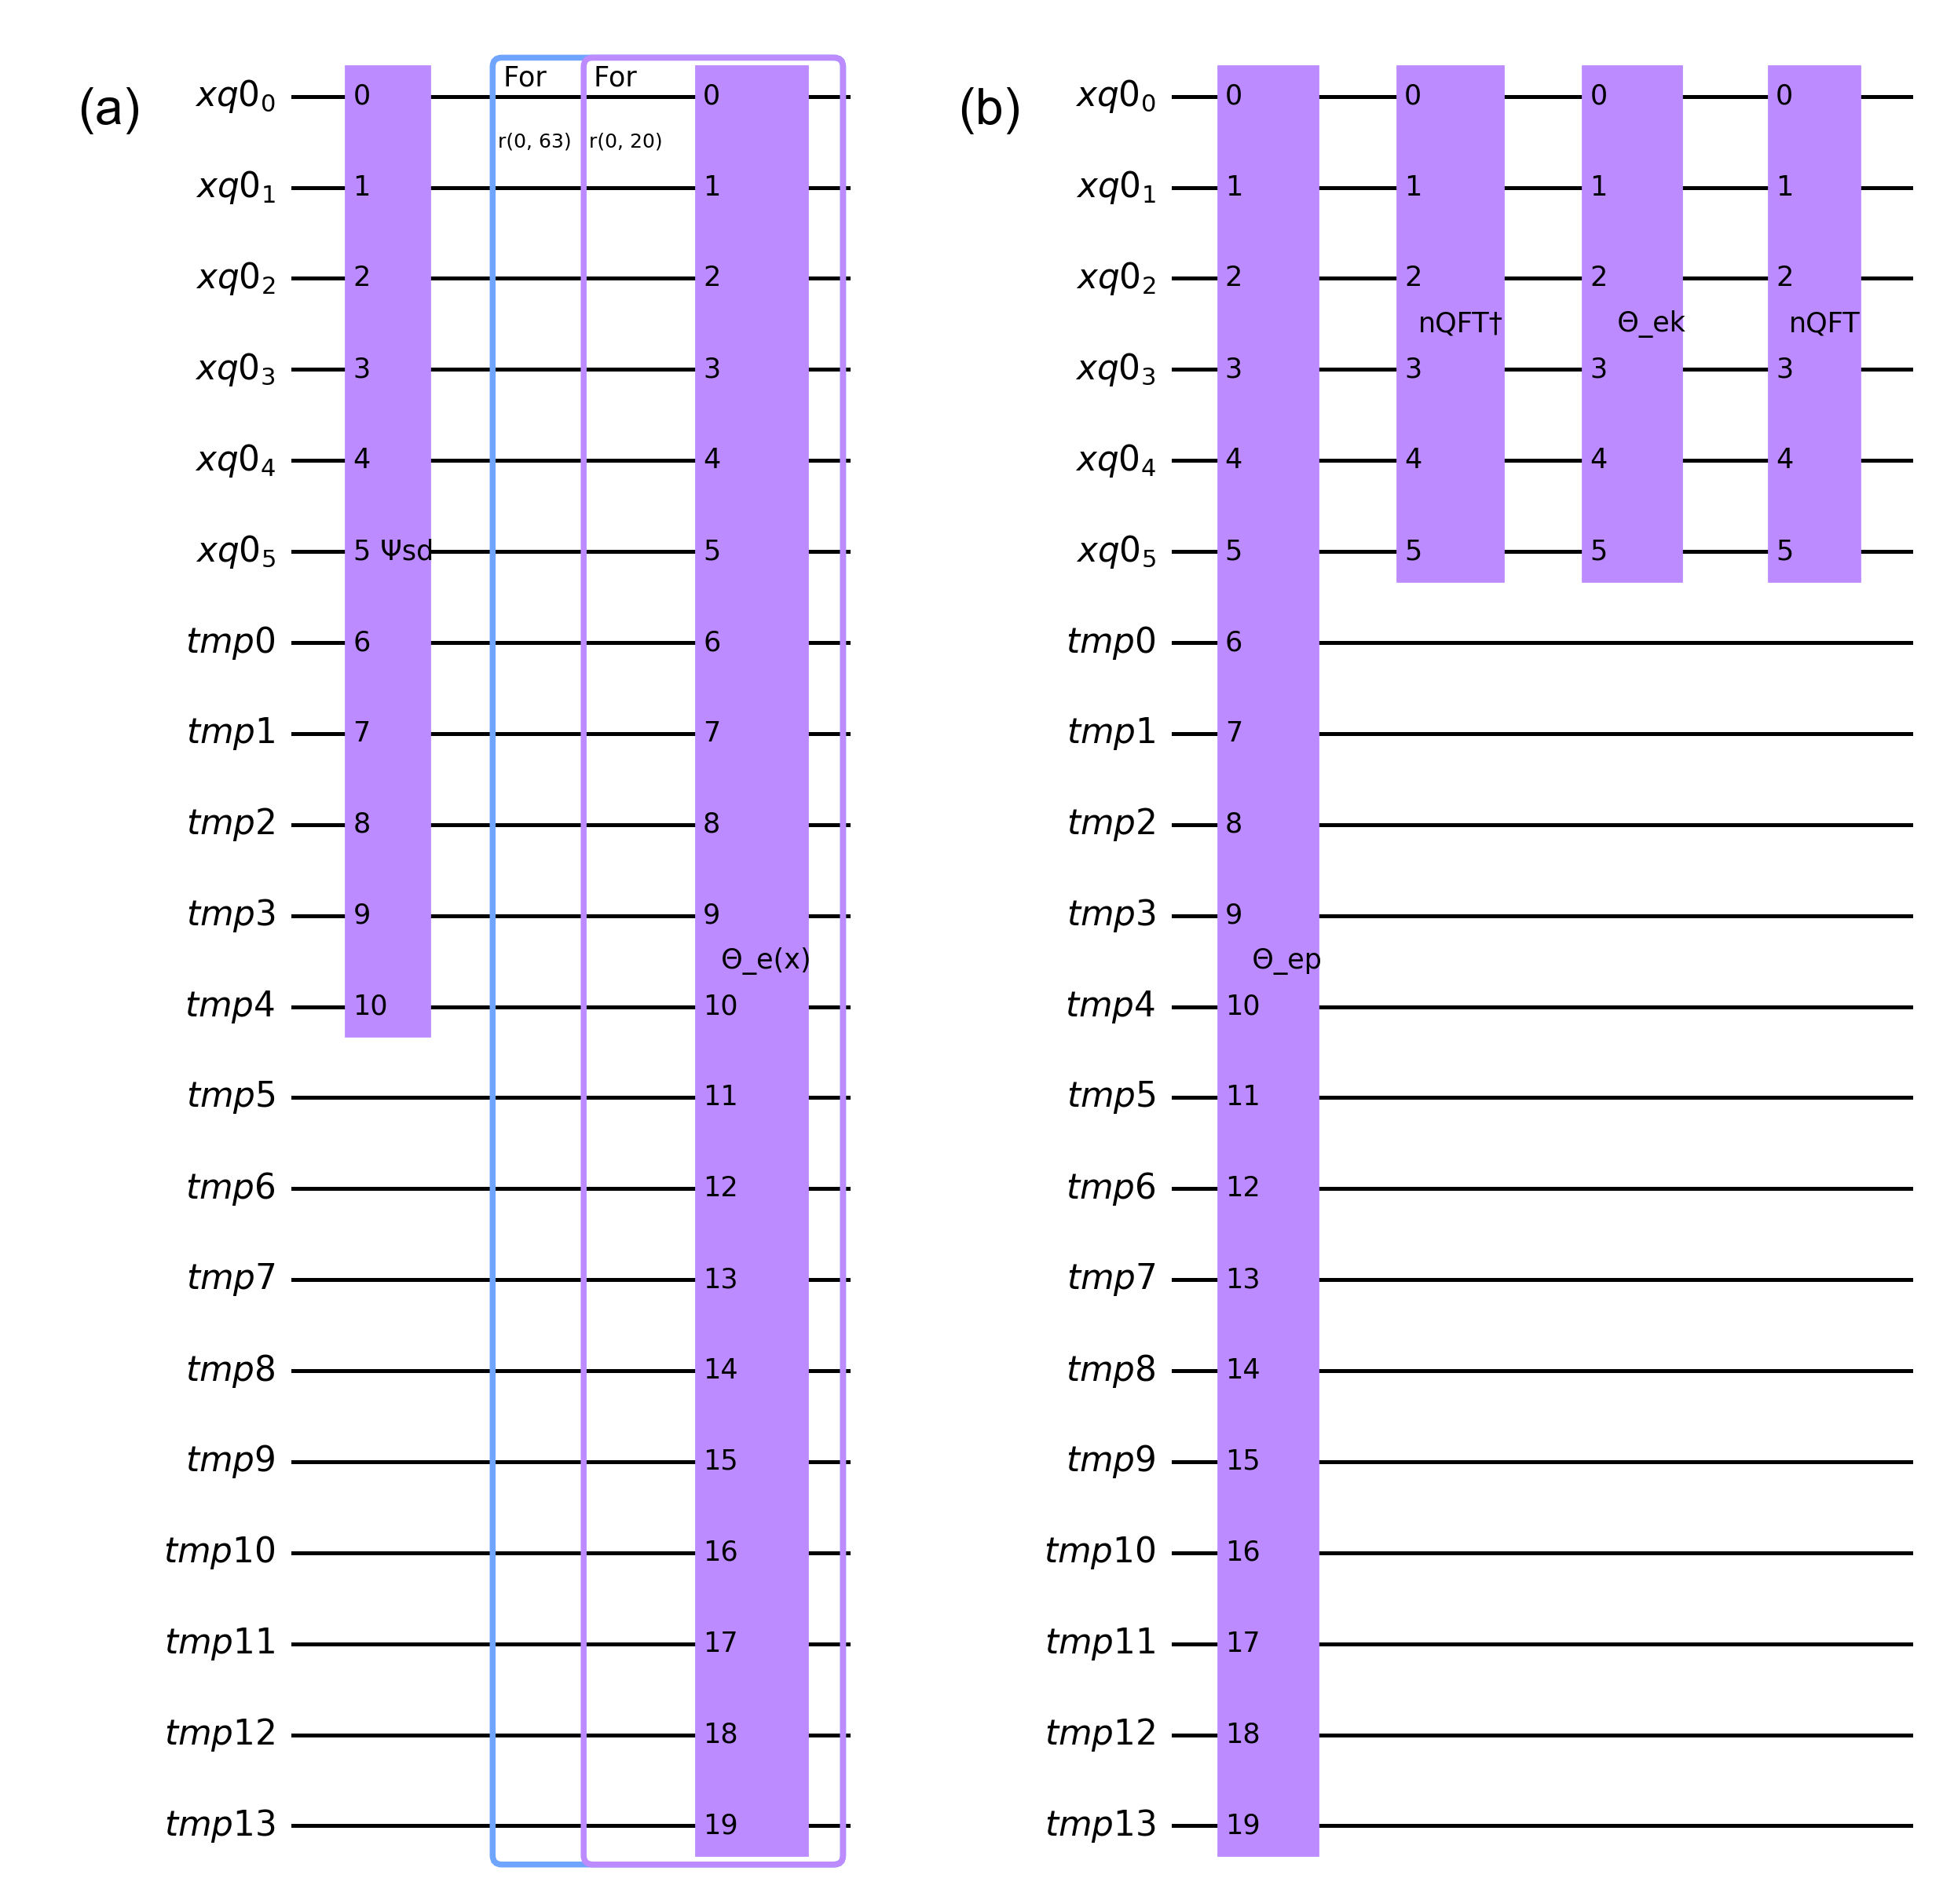
\includegraphics[width=0.72\textwidth]{paper2025_figs/arith1D/circuit_and_elec_motion.png}
    \caption{Simulator circuit of the 1D model using arithmetic operation gates}
    \label{fig:circuit-1d-arith}
    \begin{flushleft}\small

        (a) Overall view of the simulator circuit for the 1D model. It consists
        of an initialization circuit $\PsiSD$ and a time evolution circuit
        $\Thetae$. (b) Internal configuration of the time evolution circuit
        $\Thetae$. It consists of a potential energy term circuit $\Thetaep$, an
        inverse QFT circuit, a kinetic energy term circuit $\Thetaek$, and a QFT
        circuit. The number of qubits in $\Thetaep$ (23 qubits) dictates the
        total number of qubits in the entire circuit.
    \end{flushleft}
\end{figure}

\begin{figure}[ht]
    \centering
    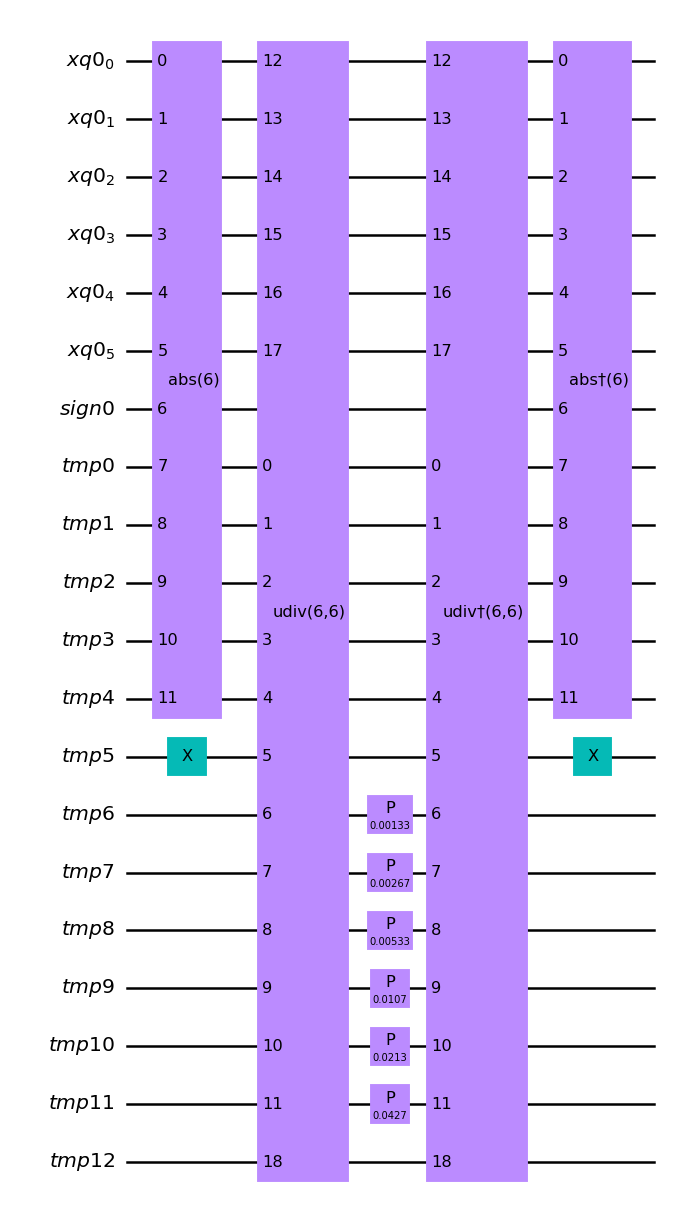
\includegraphics[width=0.5\textwidth]{paper2025_figs/arith1D/elec_potential_arithmetic.png}
    \caption{Potential energy term circuit $\Thetaep$ using arithmetic operation gates}
    \label{subfig:potential-energy-circuit-1d-arith}
    \begin{flushleft}\small

        Internal structure of the Coulomb potential term circuit $\Thetaep$
        implemented using arithmetic operation gates. It calculates $1/|x|$ in
        binary via arithmetic operations and changes the phase with a P gate
        according to the weight of the resulting bit string. The number of
        qubits in the division gate (udiv7) is dominant, and the total number of
        auxiliary qubits is 17.
    \end{flushleft}
\end{figure}

\subsubsection{Circuit Configuration Using UCRZ Circuits}
\label{subsubsec:ucrz-circuit-configuration-results}
On the other hand, the configuration using UCRZ (Uniformly Controlled Rotation
Z) circuits for calculating the Coulomb potential stayed within the emulator's
limits for the 1D and 2D models, but did not fit for the 3D model.

Figure \ref{fig:circuit-2d-ucrz} shows the configuration of the simulator using
the UCRZ circuit for the 2D hydrogen atom model. Unlike the arithmetic circuit,
the number of qubits for the potential calculation circuit $\Thetaepucr$ is kept
down to 13, and it is no longer the determining factor for the total number of
qubits in the overall circuit. In this configuration, the state preparation
circuit $\PsiSD$ for the wave function requires the most qubits.

\begin{figure}[ht]
    \centering
    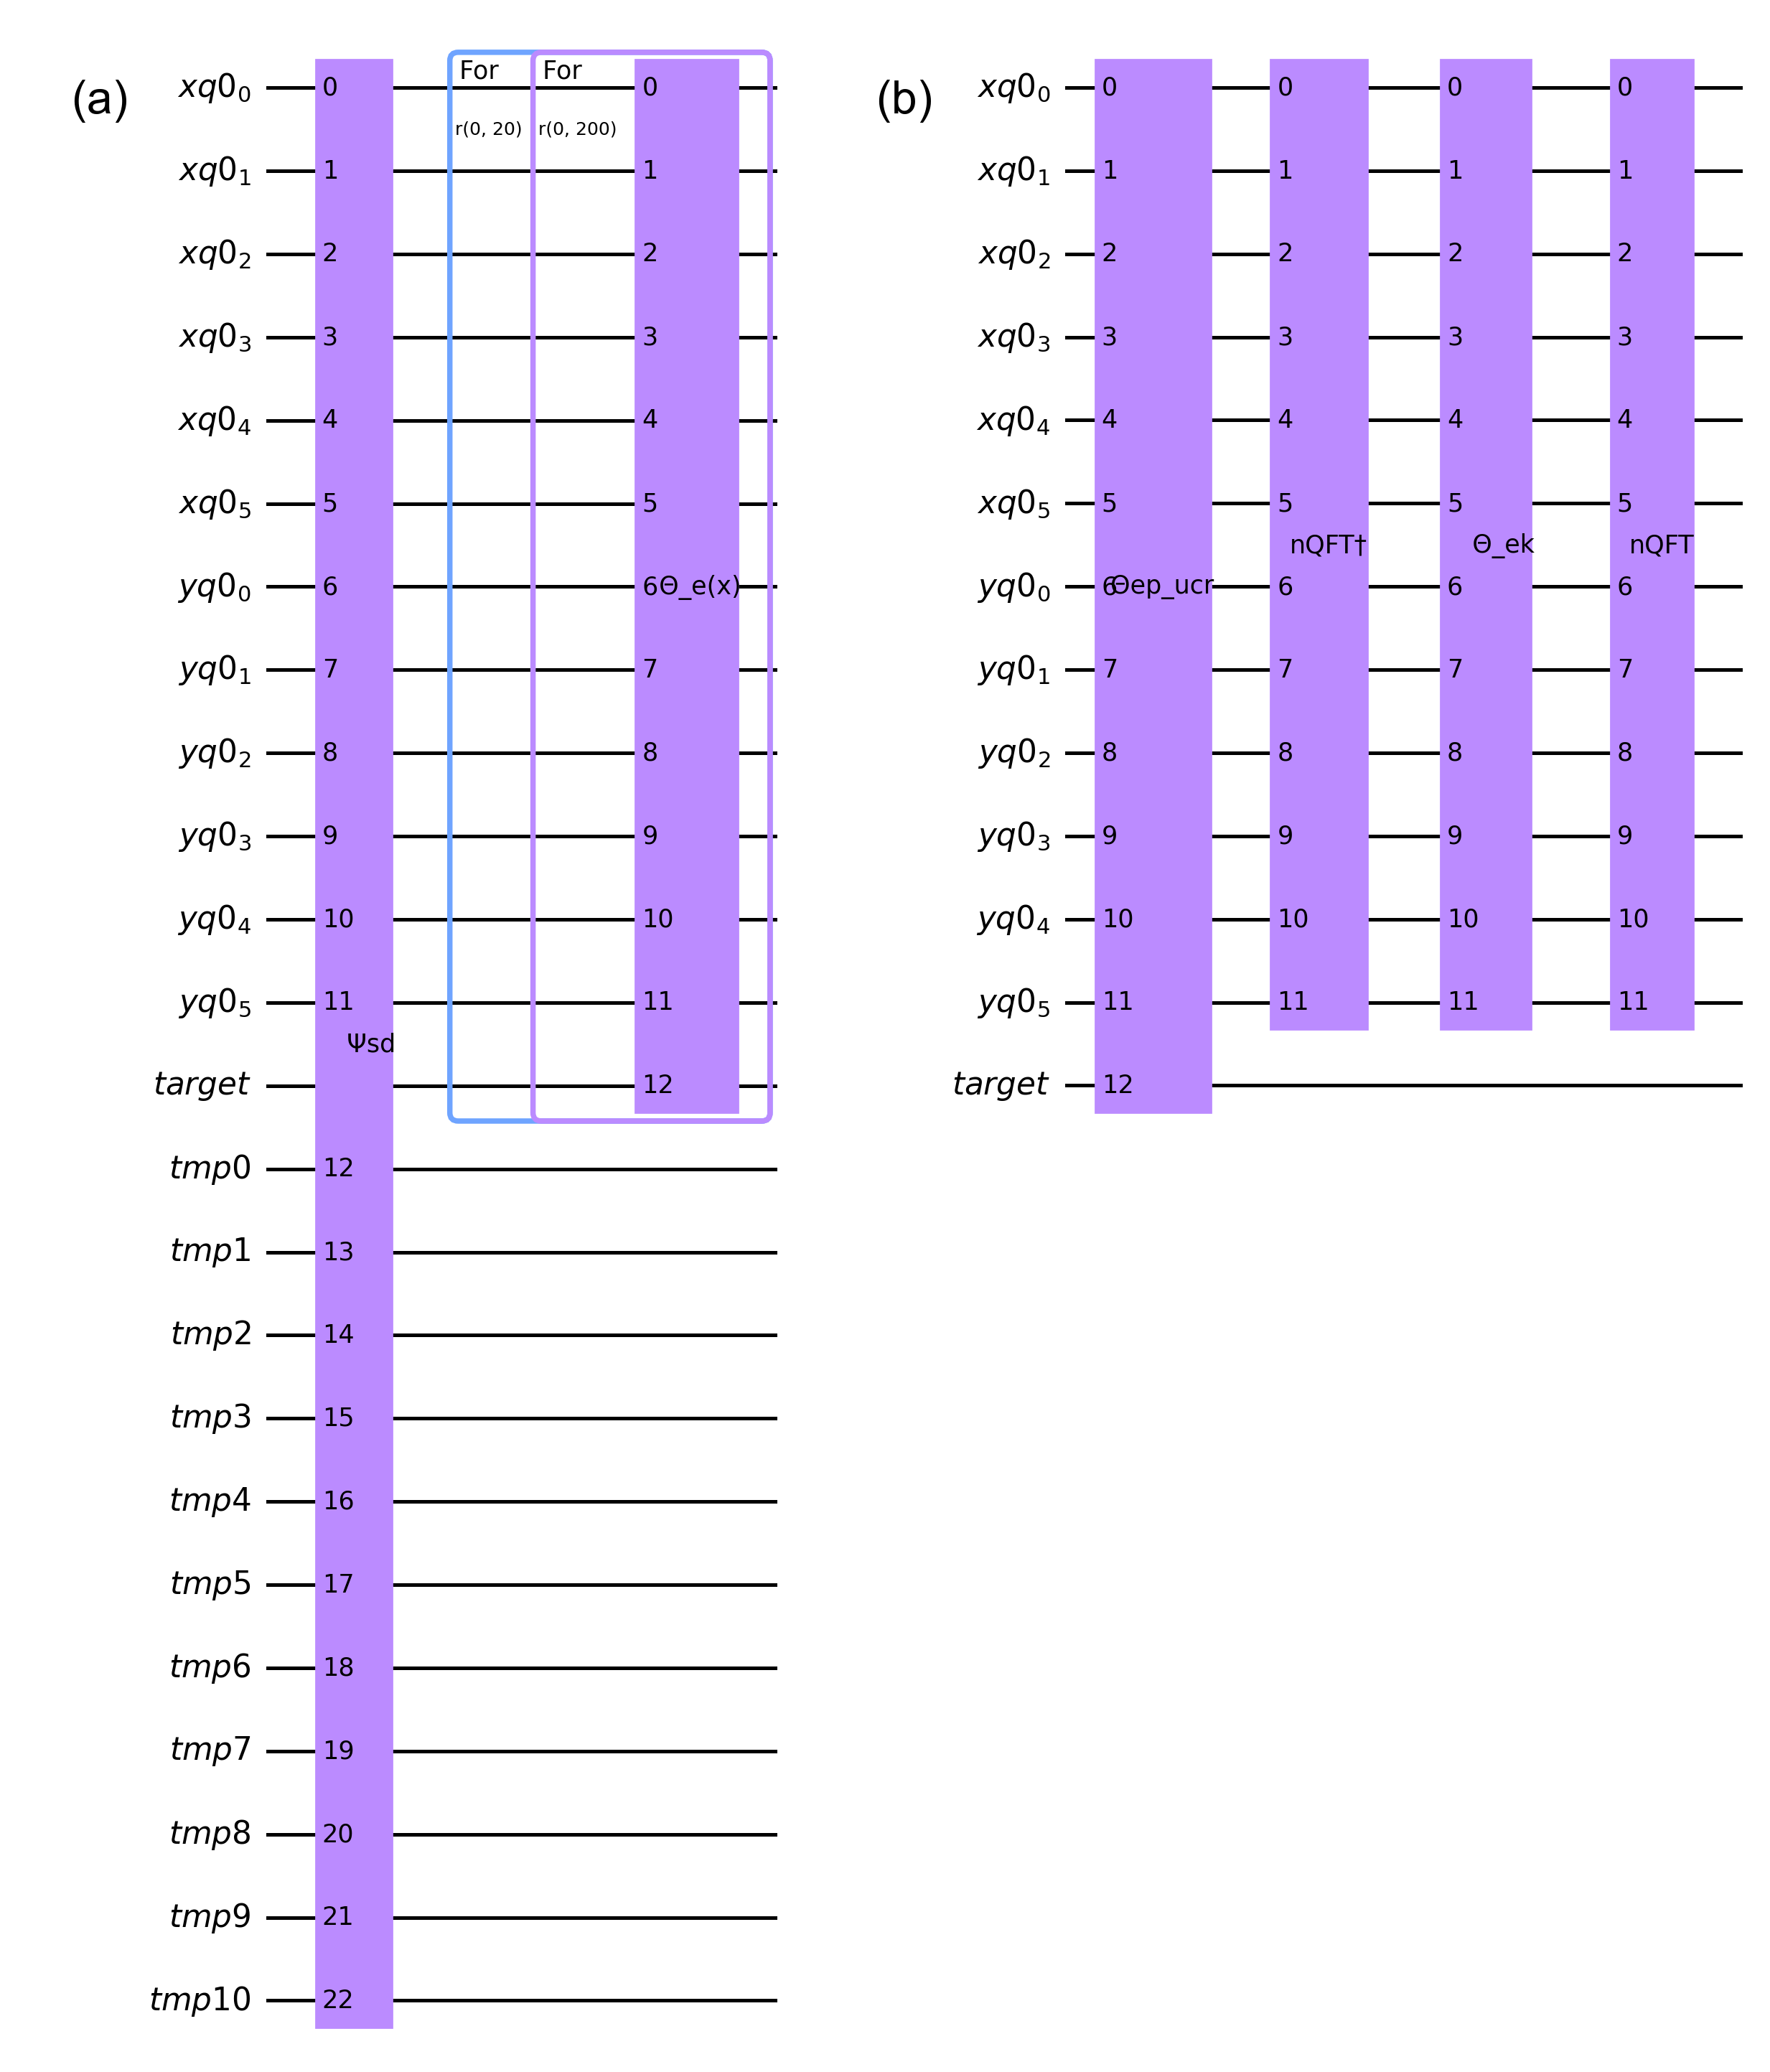
\includegraphics[width=0.72\textwidth]{paper2025_figs/ucrz2D/circuit_and_elec_motion.png}
    \caption{Simulator circuit of the 2D model with a coordinate resolution of 6 bits using UCRZ circuits}
    \label{fig:circuit-2d-ucrz}
    \begin{flushleft}\small

        (a) Overall view of the simulator circuit. The number of qubits is
        dominated by the state preparation circuit. (b) Configuration of the
        time evolution circuit. The potential energy term circuit $\Thetaepucr$
        uses a UCRZ circuit. In this example, the phase of the sole auxiliary
        qubit, $target$, is changed according to the values of the input
        registers $xq0$ and $yq0$ (6 bits each, 12 bits in total).
    \end{flushleft}
\end{figure}

\clearpage
\subsubsection{Evaluation of Circuit Size}
\label{subsec:circuit-size-evaluation-results}
In the computing environment (emulator) used in this study, the realistic
operational limits are a maximum of 27 qubits and roughly $10^7$ gates. Under
these constraints, circuits were generated using both arithmetic gate and UCRZ
gate implementations, and the scaling of the circuit size (number of qubits and
number of gates) against dimensionality and coordinate resolution was evaluated.

Figure \ref{fig:hamiltonian-gatecount} shows a comparison of the number of
qubits and 2-qubit gates (assuming 1000 time evolution steps) depending on the
implementation method of the potential circuit $\Thetaep$. Regarding the number
of qubits (top), the arithmetic circuit can be implemented with a small number
of qubits in the 1D model because only an absolute value calculation is needed.
However, in 2D and 3D models, the circuit becomes complex because norm
calculations using squares and square roots are required, causing a sharp
increase in the number of qubits. As a result, the arithmetic circuit fits
within the emulator limit (27 qubits) only for 1D models at 7 bits or less.
Conversely, the UCRZ circuit was confirmed to stay within the qubit limit up to
an 8-bit resolution in 3D.

On the other hand, focusing on the number of gates (bottom), the trend reverses.
While the number of gates in the arithmetic circuit increases only moderately as
dimensionality increases, the number of gates in the UCRZ circuit increases
exponentially with respect to the number of input bits (dimensionality $\times$
coordinate bits). Consequently, the UCRZ circuit has fewer gates for 1D models
and 2D models with 6 or fewer coordinate bits, but for 3D models, the arithmetic
circuit requires fewer gates than the UCRZ circuit across all bit counts.

\begin{figure}[ht]
    \centering
    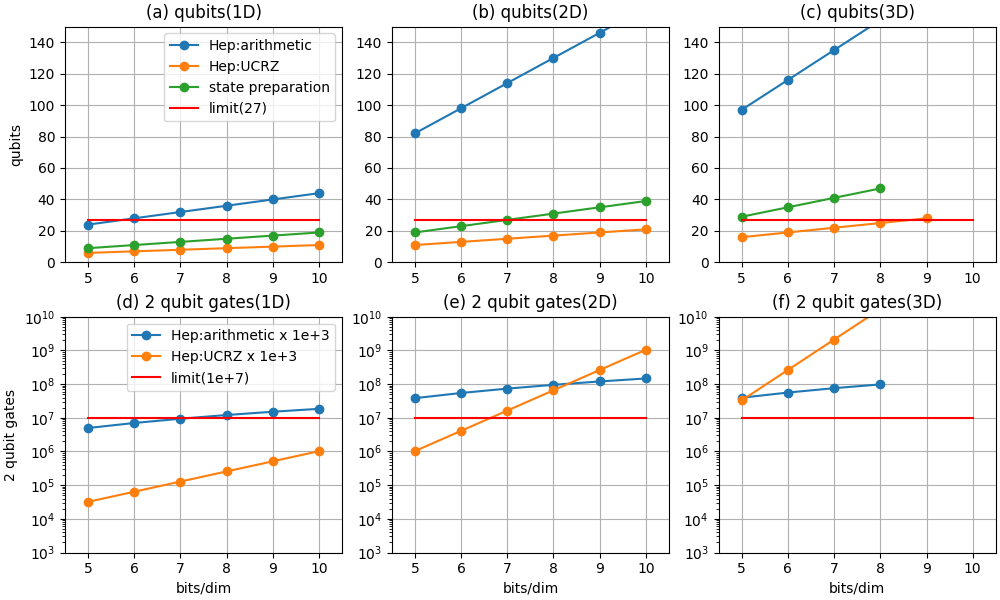
\includegraphics[width=15cm]{paper2025_figs/hamiltonian-gatecount-revision2.png}
    \caption{Circuit Size}
    \label{fig:hamiltonian-gatecount}
    \begin{flushleft}\small

    Top: Required number of qubits in 1D-3D models. The arithmetic circuit stays
    within the limit (black dashed line) only in 1D (7 bits or less), while the
    UCRZ circuit stays within the limit up to 3D (8 bits). The sharp increase in
    qubits for arithmetic circuits in 2D/3D is due to the complexity of norm
    calculations. 
    
    Bottom: Number of 2-qubit gates required for 1000 steps of time evolution.
    The arithmetic circuit shows moderate growth against dimensionality, whereas
    the UCRZ circuit increases exponentially against input bits, making the
    arithmetic circuit more advantageous in terms of gate counts in a 3D
    environment.
    \end{flushleft}
\end{figure}

From these evaluations, it was shown that when actually running circuits on a
quantum computer (or emulator), it is necessary to select the optimal
implementation method by considering the trade-off between the dimensionality of
the target model and the available number of qubits and gates (coherence time).
Table \ref{tab:emulator-circuit-configurations} summarizes the combinations of
circuit configurations that were actually operable under this emulator
environment.

\begin{table}[ht]
\centering
\caption{List of circuit configurations operable on the emulator}
\begin{tabular}{rcc}
    \hline
    Dimensionality & $\nb$ for arithmetic gate circuit & $\nb$ for UCRZ circuit \\
    \hline
    1 & 6,7 & Not evaluated (operated with arithmetic operations) \\
    2 & Did not operate & 6 \\
    3 & Did not operate & Did not operate \\
    \hline
\end{tabular}
\label{tab:emulator-circuit-configurations}
\end{table}

Under the conditions in Table \ref{tab:emulator-circuit-configurations}, by
applying the Coulomb potential singularity treatment formulated in Section
\ref{sec:coulomb-potential-handling} and setting the optimal simulation
parameters derived in Section \ref{sec:parameter-selection-for-minimum-error},
the expected time evolution of the wave function was confirmed using either the
arithmetic circuit or the UCRZ circuit. Detailed analyses of the obtained
calculation errors will be described in the following subsections.

\begin{figure}[ht]
    \centering
    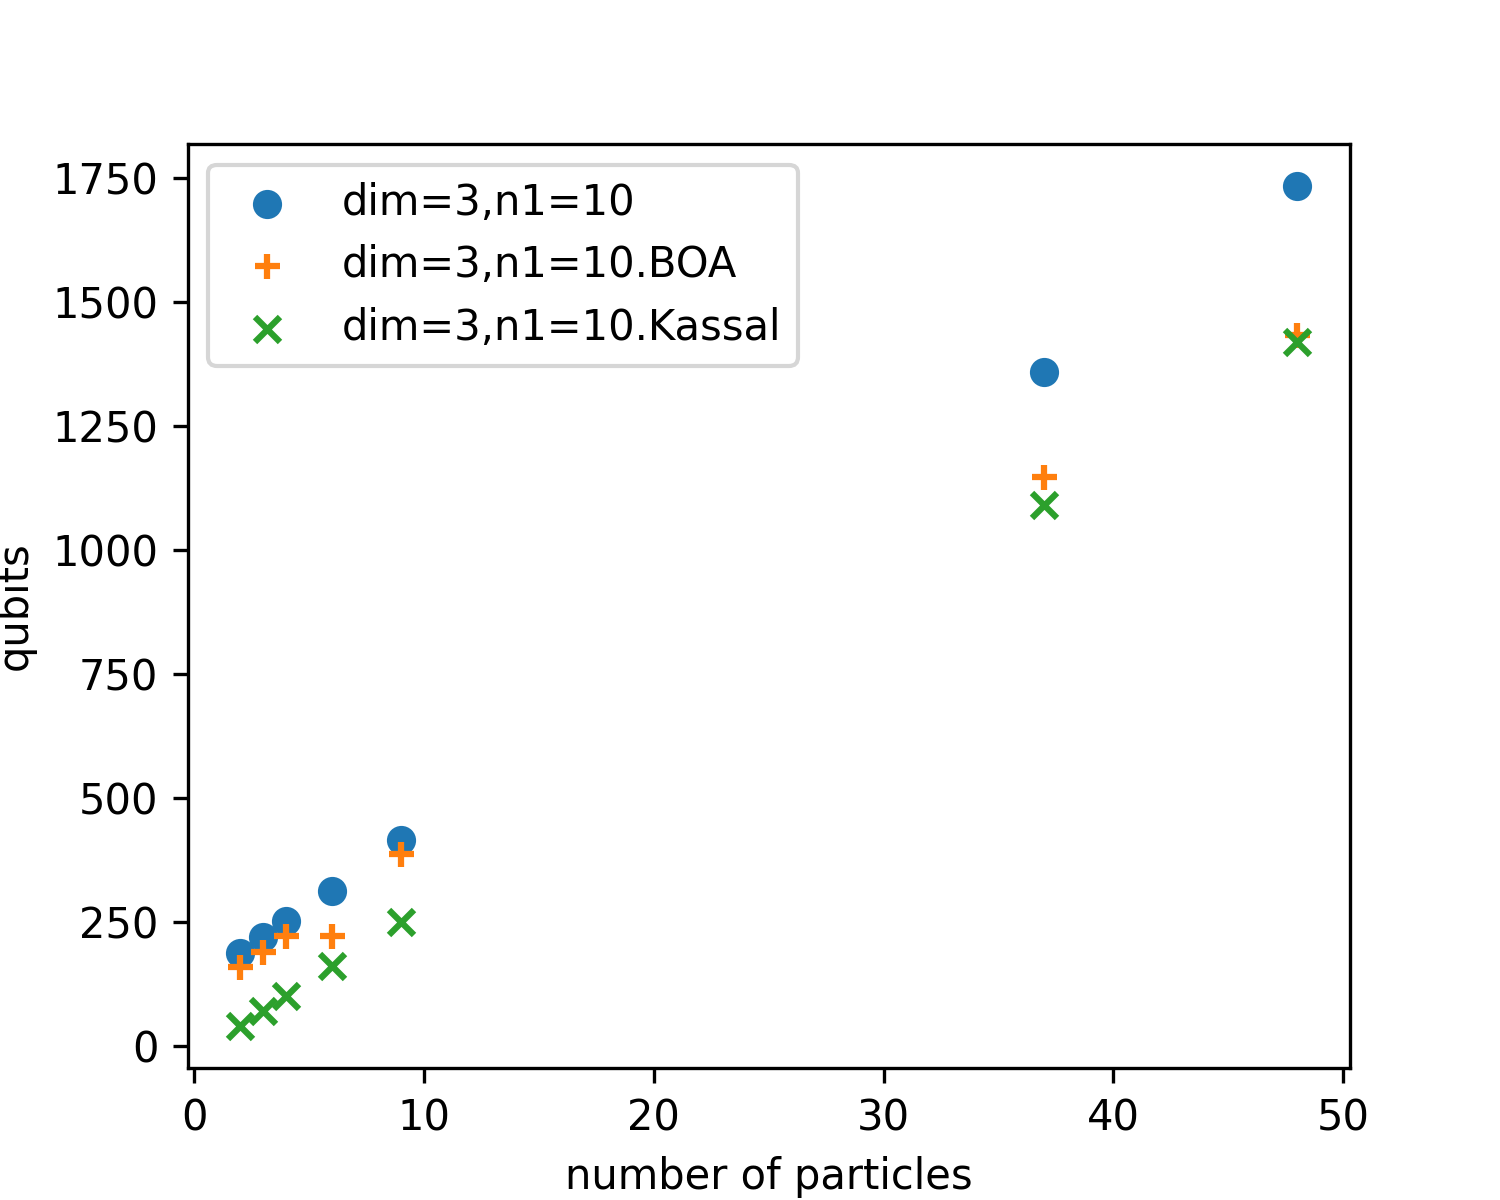
\includegraphics[width=0.6\textwidth]{paper2025_figs/circuit-size-qubits.png}
    \caption{Relationship between the number of particles and the number of qubits}
    \label{fig:qubit-for-some-molecules}
    \begin{flushleft}\small

        The horizontal axis is the number of particles (number of electrons +
        number of nuclei), and the vertical axis is the required number of
        qubits when using an arithmetic circuit (3D, 10-bit coordinates). Each
        point from left to right indicates \ce{H}, \ce{He}, \ce{Li}, \ce{H +
        H2}, \ce{O}, Glycine (\ce{C2H5NO2}), and Alanine (\ce{C3H7NO2}).
        ``\verb|+|'' indicates the case where the nuclear positions are fixed
        (Born-Oppenheimer approximation). ``\verb|x|'' indicates values based on
        the estimation formula by Kassal et al.
        \cite{kassal2008.pnas.0808245105}.
    \end{flushleft}
\end{figure}

Finally, anticipating execution on future large-scale quantum computers, we
ignored emulator limits, generated the proposed arithmetic circuit (3D, 10-bit
resolution) for various atomic and molecular models, and evaluated scalability.
As shown in Figure \ref{fig:qubit-for-some-molecules}, it is confirmed that the
required number of qubits scales linearly with respect to the number of
particles in the system (sum of electrons and nuclei).

\subsection{Handling the Pole of the Coulomb Potential}
\label{subsec:coulomb-potential-handling-results}
In this subsection, we present energy evaluation results for the divergence
avoidance methods at the singularity (pole) of the Coulomb potential formulated
in Section \ref{sec:coulomb-potential-handling}, using the local average
potential and the soft-core potential, respectively.

\subsubsection{Method Using Local Average Potential}
\label{subsubsec:local-average-potential-results}

In the local average potential $\Hla(r)$ defined in Equation \eqref{eq:Halr}, we
set the effective distance to $\reff = \deltar/a$ and evaluated the calculated
energy values against multiple qubit numbers $\nb$ while varying the coefficient
$a$ in the range of $1 \le a \le 8$. Note that since this evaluation includes
parameters that exceed the emulator's limits (qubit upper limit), the
calculations were performed using a classical simulation program that performs
operations equivalent to the behavior of the quantum circuit.

The evaluation results for the 2D model wave functions $\PsiTwoD_{0,0}$ and
$\PsiTwoD_{1,0}$ are shown in Figures \ref{fig:Ha1-vs-delta1}(a) and (b),
respectively. As is clear from the graphs, for both states, when setting $a=4$,
i.e., $\reff = \deltar/4$, the energy expectation values most closely matched
the analytical solutions ($-2.0\ \mathrm{a.u.}$ and $-0.2222\ \mathrm{a.u.}$,
respectively).

At any resolution (number of bits), the sign of the error reverses around $a=4$,
confirming that the optimal condition is common and independent of the number of
bits. This strongly supports the validity of the theoretical approximation in
Section \ref{sec:coulomb-potential-handling}, which derived $\reff \approx
\deltar/4$ from the consistency of the integral value in a minute region.

\begin{figure}[ht]
    \centering
    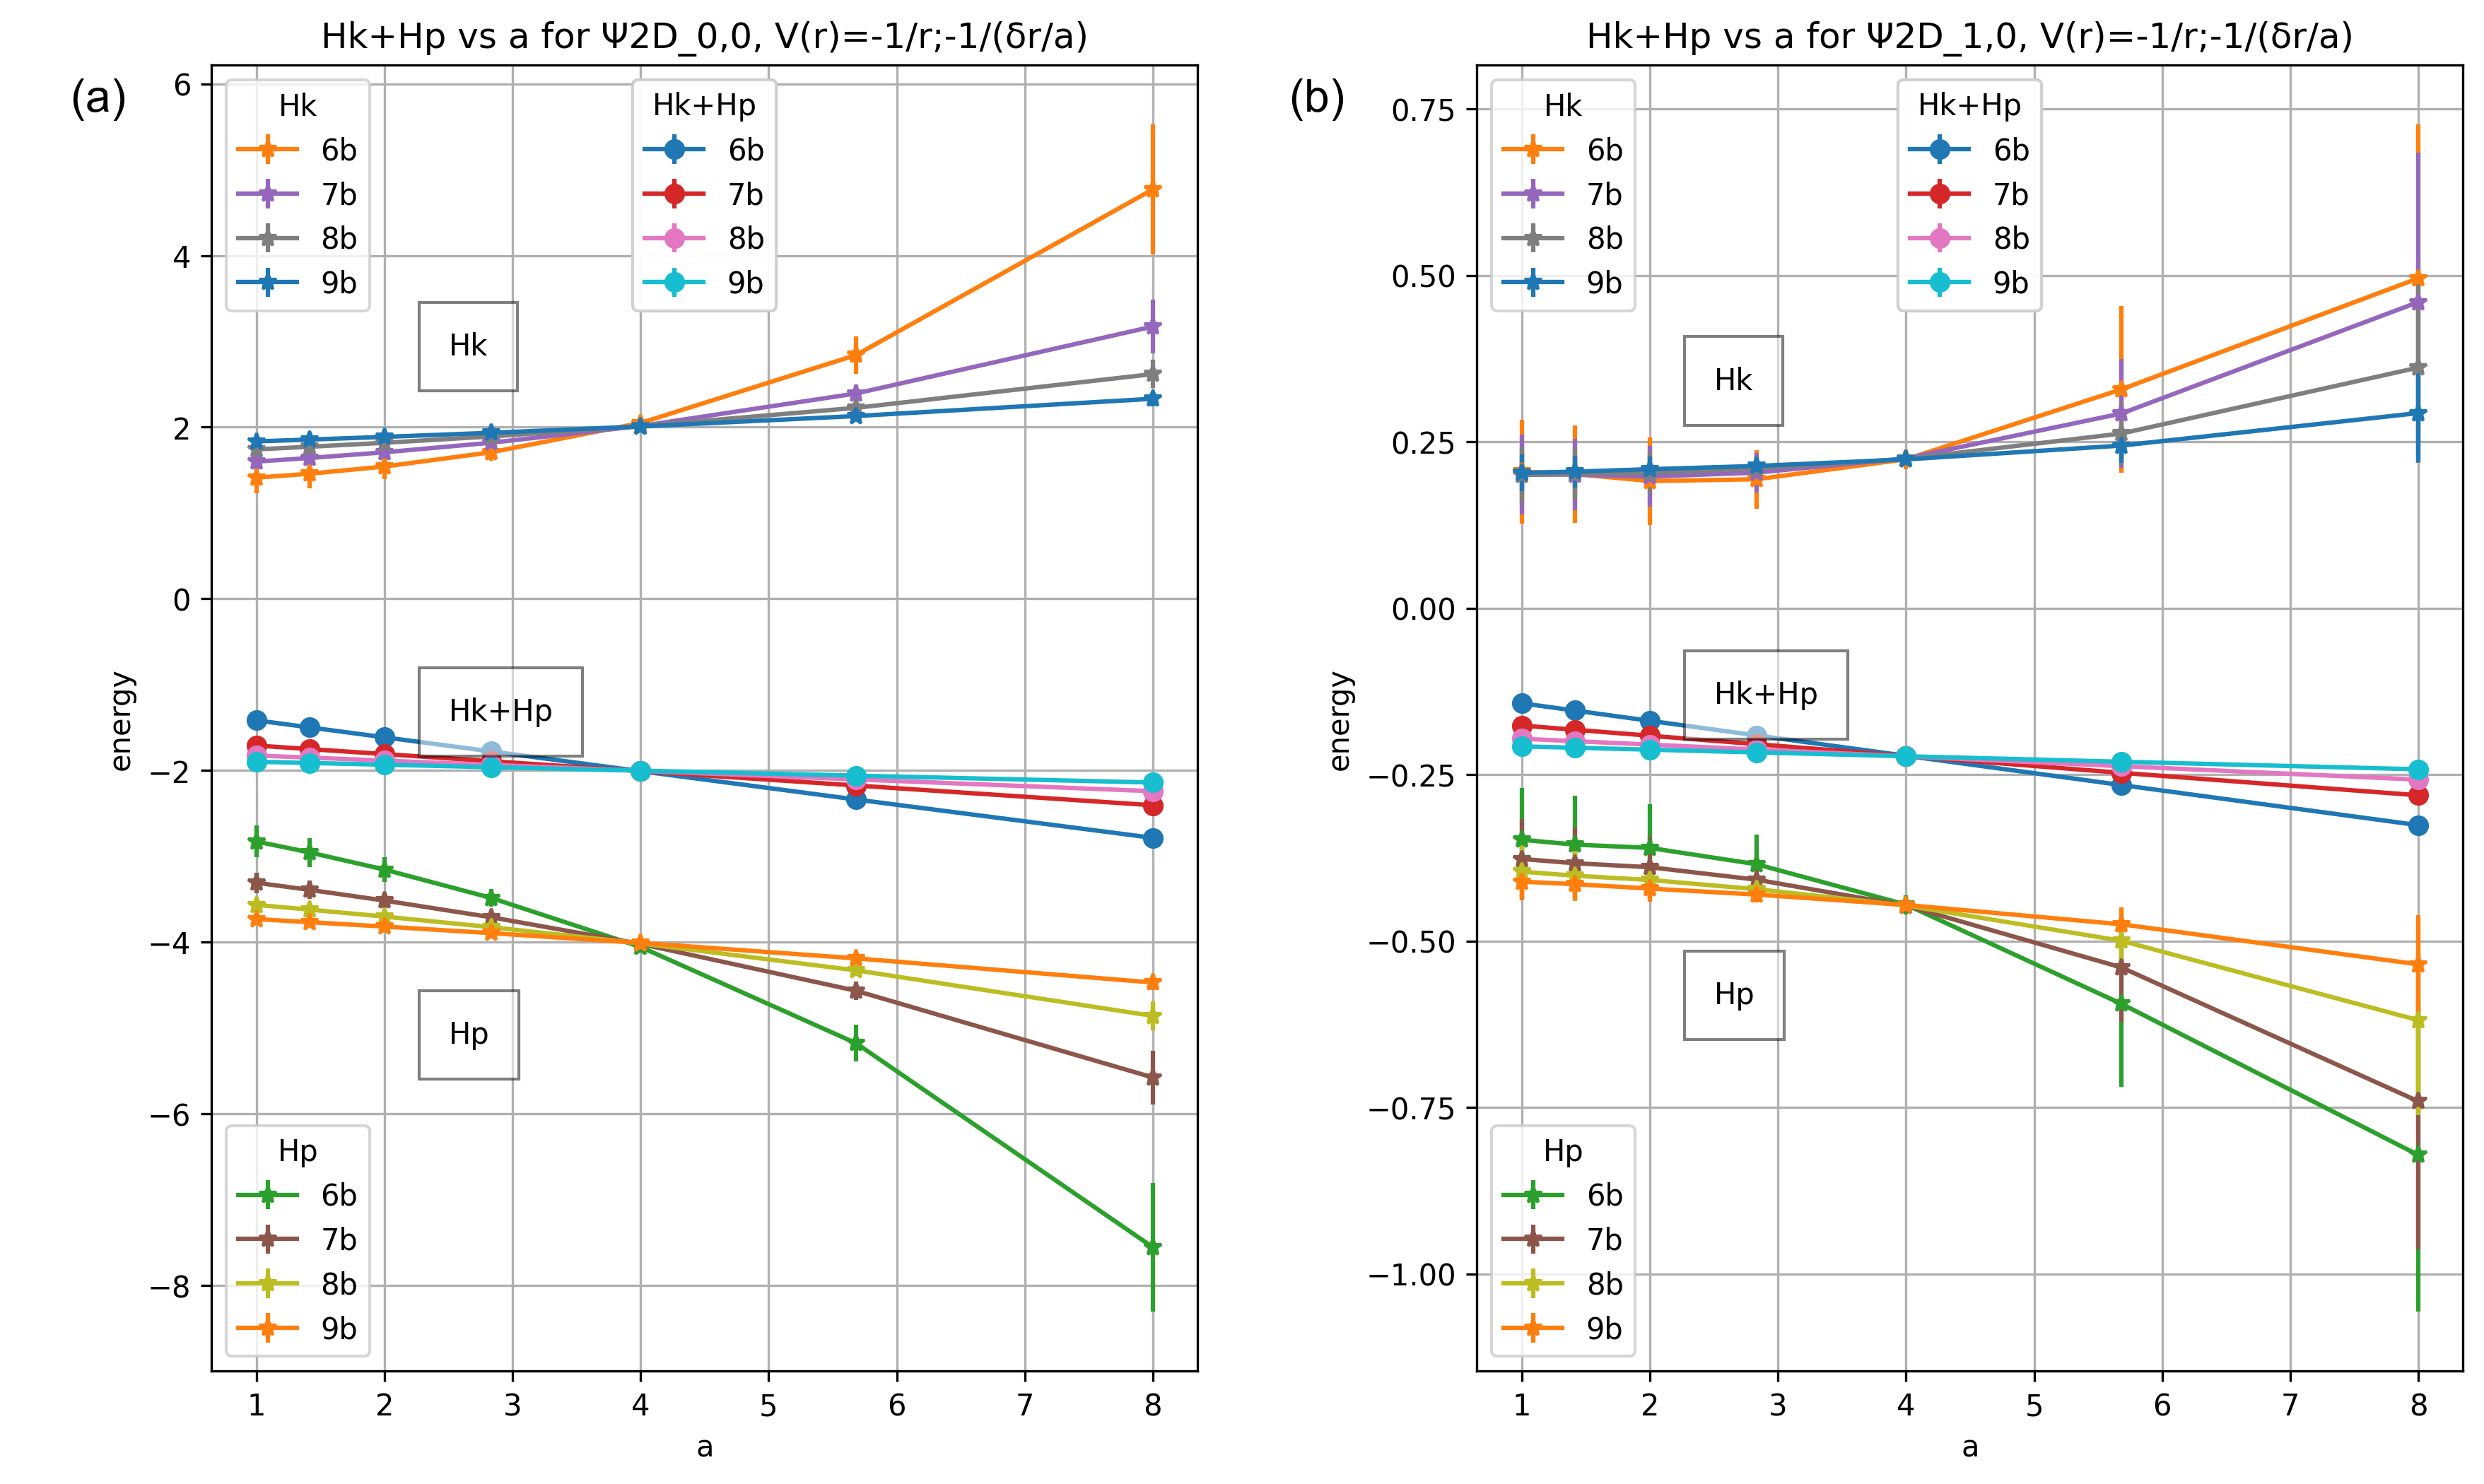
\includegraphics[width=0.95\columnwidth]{paper2025_figs/compare_energy/compare_energy_h2D_TO2_r0lim_combined.png}
    \caption{Changes in energy values when varying $\reff$ in the approximation formula $\Hla(r)$}
    \label{fig:Ha1-vs-delta1}
    \begin{flushleft}\small

        (a) Graph for state $\PsiTwoD_{0,0}$ setting $\reff=\deltar/a$ and
        varying $a$. The horizontal axis $a$ is a geometric progression with a
        ratio of $\sqrt{2}$. At all bit counts, when $a=4$ ($\reff=\deltar/4$),
        the expectation value of the Hamiltonian $\Hk+\Hp$ closely approaches
        the analytical solution of $-2.0$. (b) Results for state
        $\PsiTwoD_{1,0}$. Similarly, the value is closest to the analytical
        solution $-0.2222$ at $a=4$.
    \end{flushleft}
\end{figure}

\subsubsection{Soft-Core Potential}
\label{subsubsec:soft-core-potential-results}
Next, for the soft-core potential $\Hsc(r)$ defined in Equation
\eqref{eq:Hsc2r}, Figure \ref{fig:Ha2-vs-delta2} shows the calculated energy
values when setting the offset constant to $\Delta = \deltar/a$ and varying $a$
(the calculation method is the same as in the previous section).

The soft-core potential takes exactly the same constant form at the singularity
$r=0$ as $\Hsc(0)=-1/\Delta$, which is identical to the local average potential
$\Hla(0)=-1/\reff$. As can be seen from the results in Figure
\ref{fig:Ha2-vs-delta2}, similar to the case of $\Hla(r)$, adopting $a=4$ (i.e.,
$\Delta=\deltar/4$) yielded energy expectation values closest to the analytical
solution.

Although there are differences in the functional forms in the region of $r \neq
0$, the error in the energy expectation value is dominated by the behavior near
the singularity, which is likely why no significant difference occurred in the
overall calculated values. This result indicates that even when the soft-core
potential is used for the purpose of regularizing the singularity, the boundary
condition $\Delta = \deltar/4$ derived from the local average potential
functions as the optimal parameter.

\begin{figure}[ht]
    \centering
    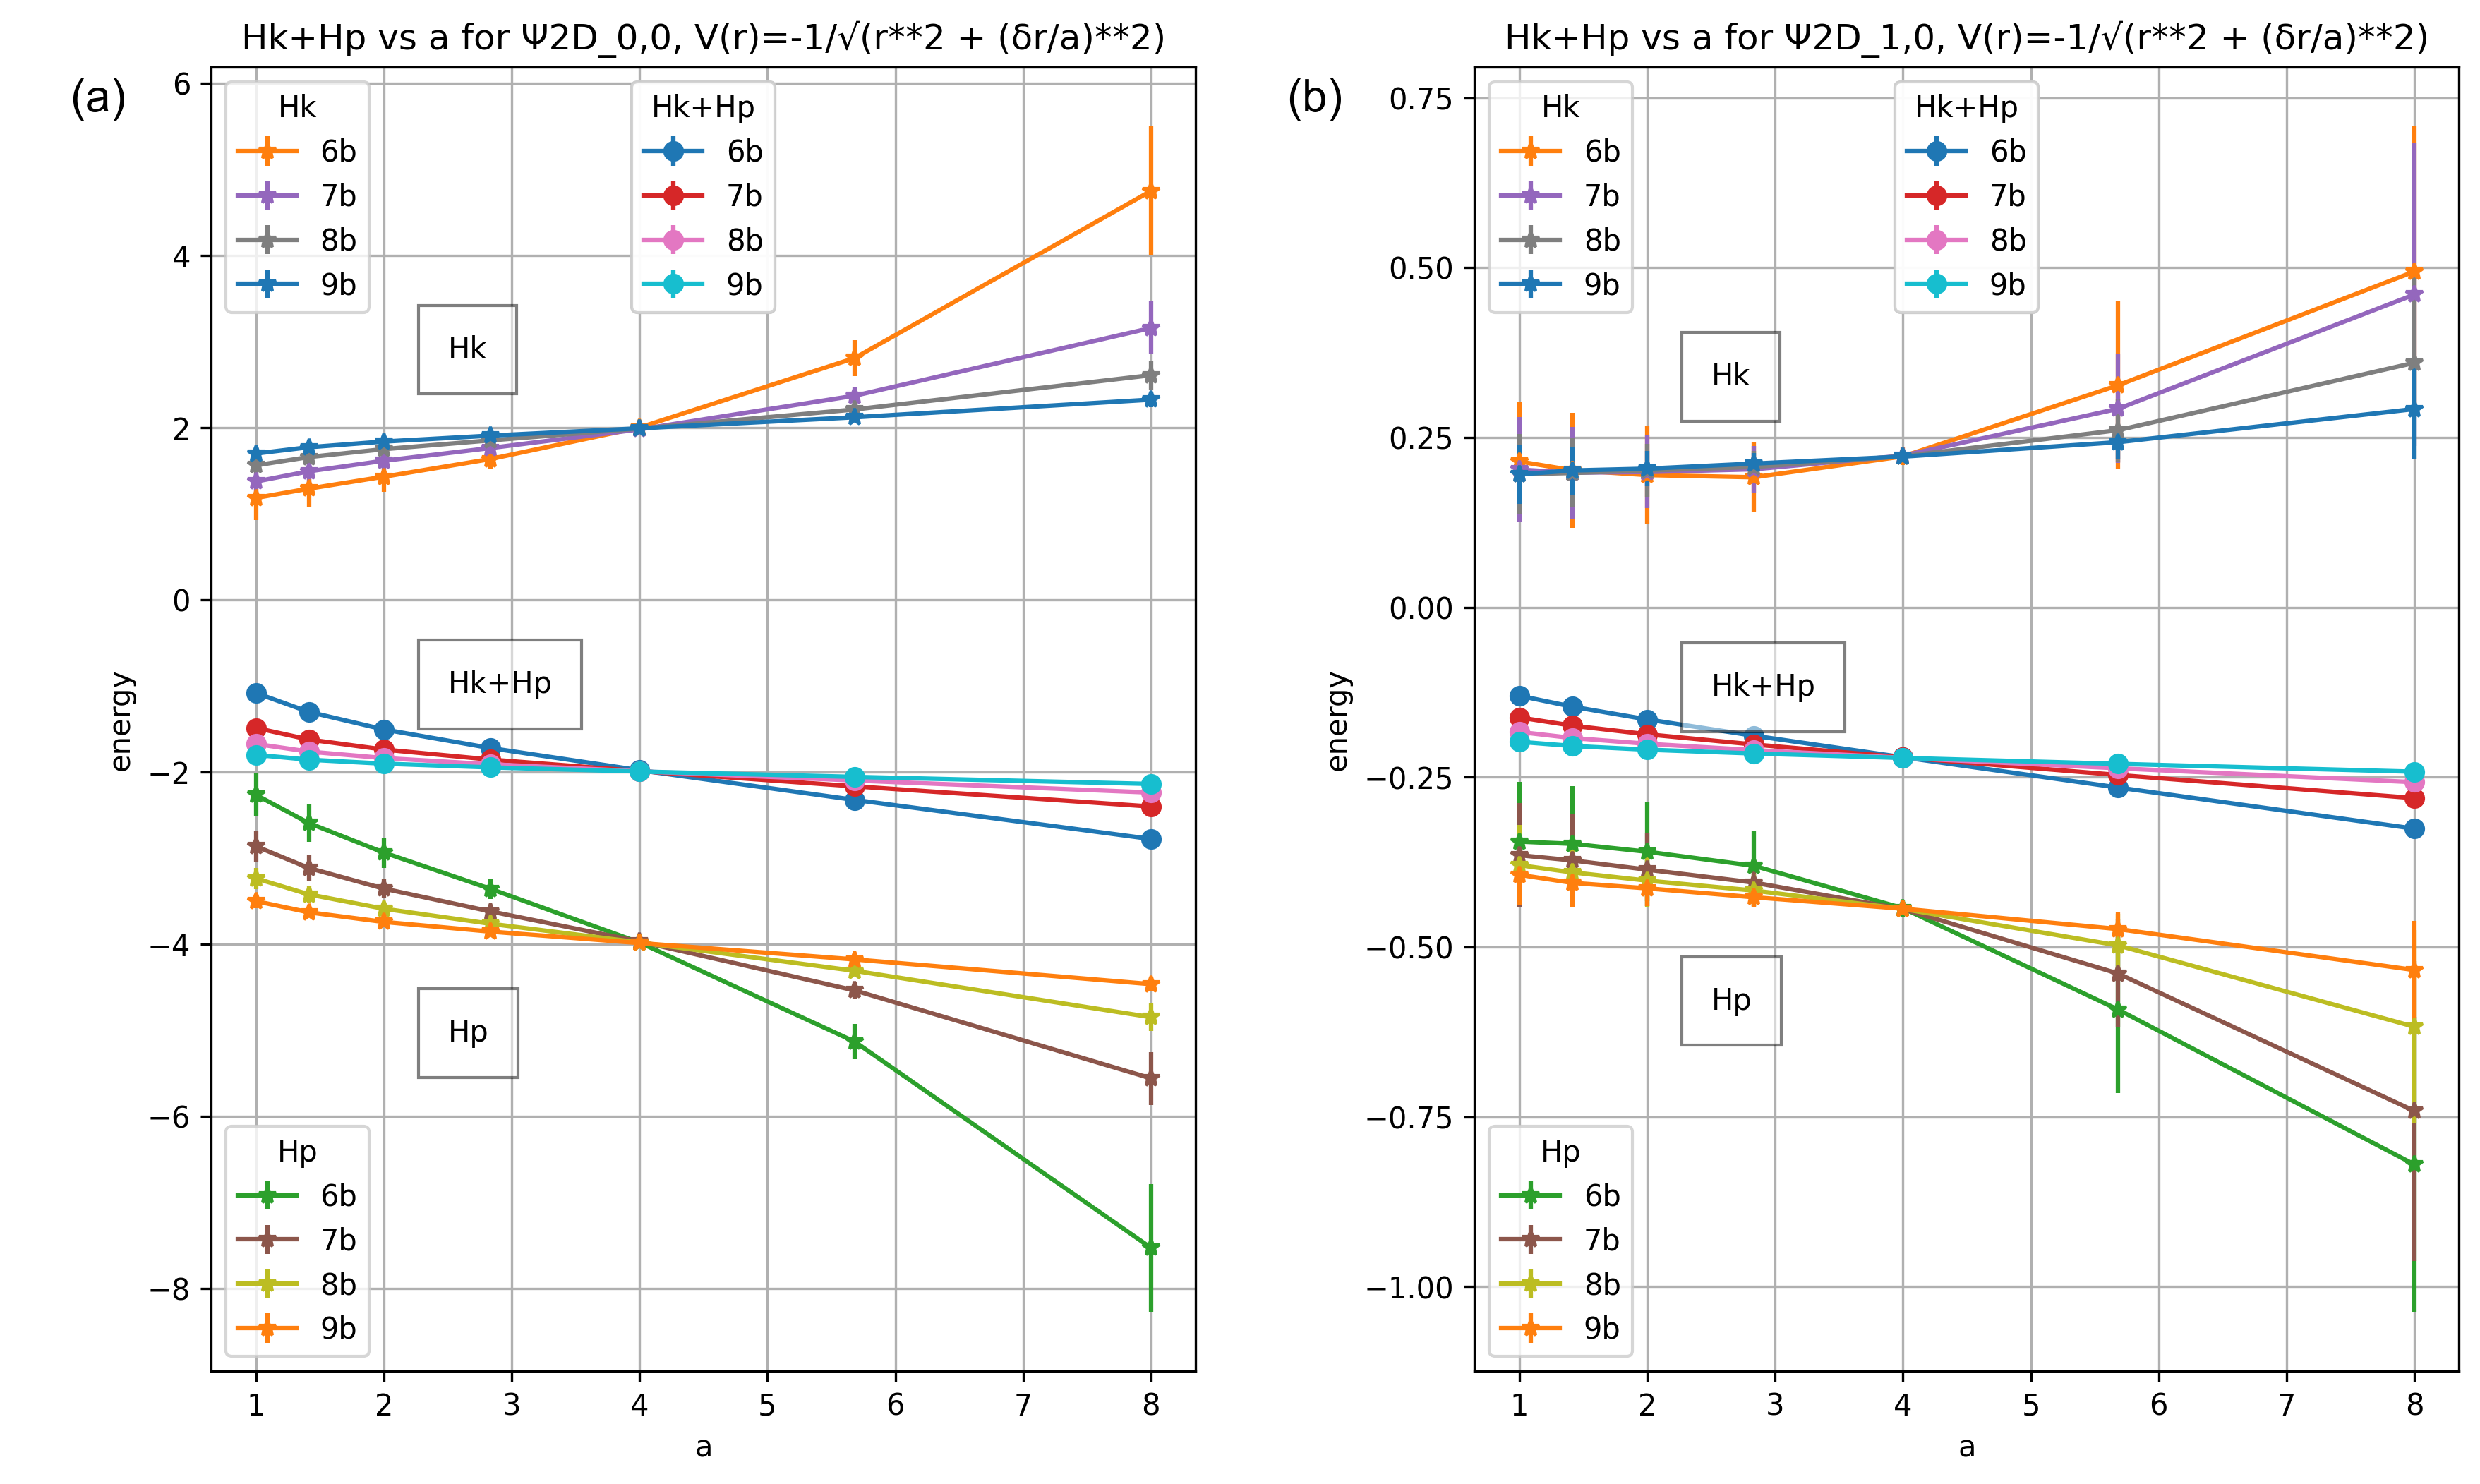
\includegraphics[width=0.95\columnwidth]{paper2025_figs/compare_energy/compare_energy_h2D_TO2_rofs_combined.png}
    \caption{Changes in energy values when varying $\Delta$ in the approximation formula $\Hsc(r)$}
    \label{fig:Ha2-vs-delta2}
    \begin{flushleft}\small

        (a) Graph for state $\PsiTwoD_{0,0}$ setting $\Delta=\deltar/a$ and
        varying $a$ ($a$ is a geometric progression with a ratio of $\sqrt{2}$).
        Across all bit counts, $\Hk+\Hp$ shows the closest value to the
        analytical solution $-2.0$ when $a=4$ ($\Delta=\deltar/4$). (b) Results
        for state $\PsiTwoD_{1,0}$. Similarly, the energy expectation value is
        closest to the analytical solution $-0.2222$ at $a=4$.
    \end{flushleft}
\end{figure}
\clearpage

\subsection{Simulation Parameters for Minimizing Error}
\label{subsec:parameter-selection-for-minimum-error-results}
In this subsection, we present the results of specific numerical evaluations
regarding the parameter determination method for minimizing errors discussed in
Section \ref{sec:parameter-selection-for-minimum-error}. First, we describe the
optimization of the grid spacing based on the trade-off between spatial
discretization error and cutoff error, and then we show the evaluation results
of the time parameter (number of divisions) based on the sampling theorem and
the Suzuki-Trotter decomposition.

\subsubsection{Method for Determining Grid Spacing}
\label{subsubsec:delta-r-selection-results}

Figure \ref{fig:dq-tradeoff}(a) shows the evaluation results of the relationship
between the spatial discretization error $\errdisc = |S_d-S_1|$ and the cutoff
error $\errcutoff = S_2$ at multiple qubit numbers $\nb$ for the 1D model wave
function $\PsiOneD_1$.

Focusing on the case with the smallest number of qubits, $\nb=6$, the curves for
$\errcutoff$ and $\errdisc$ intersect around $\deltar \approx 0.22$ in graph
(A2). This point represents the equilibrium value for the trade-off between the
two errors, corresponding to the optimal parameter where their sum in graph (A3)
takes the minimum value. At this time, the dimension of the simulation region is
$L=14$. (In (A1), the real part of the wave function amplitude and the boundary
positions of $\pm L/2$ are indicated by vertical lines.)

On the other hand, in the case of $\nb=8$ where the number of qubits is
increased, graph (A3) shows that the range of $\deltar$ where the sum of errors
is minimized (almost zero) is wide and flat, from $0.07 \sim 0.14$. This means
that under conditions with ample computational resources such as qubit count,
the selection range for the optimal parameter broadens. Note that outside this
range, the sharp increase in error at $\deltar < 0.07$ is due to the
manifestation of the cutoff error caused by shrinking the spatial size $L$,
while the increase in error at $\deltar > 0.14$ is due to an increase in spatial
discretization error caused by coarse spatial resolution.

Figures \ref{fig:dq-tradeoff}(b) and (c) show the results for the 2D model wave
functions $\PsiTwoD_{0,0}$ and $\PsiTwoD_{1,0}$, respectively. It can be
confirmed that the optimal range for appropriate $\deltar$ varies significantly
depending on the difference in the target states (spatial spread of the wave
functions).

\begin{figure}[ht]
    \centering
    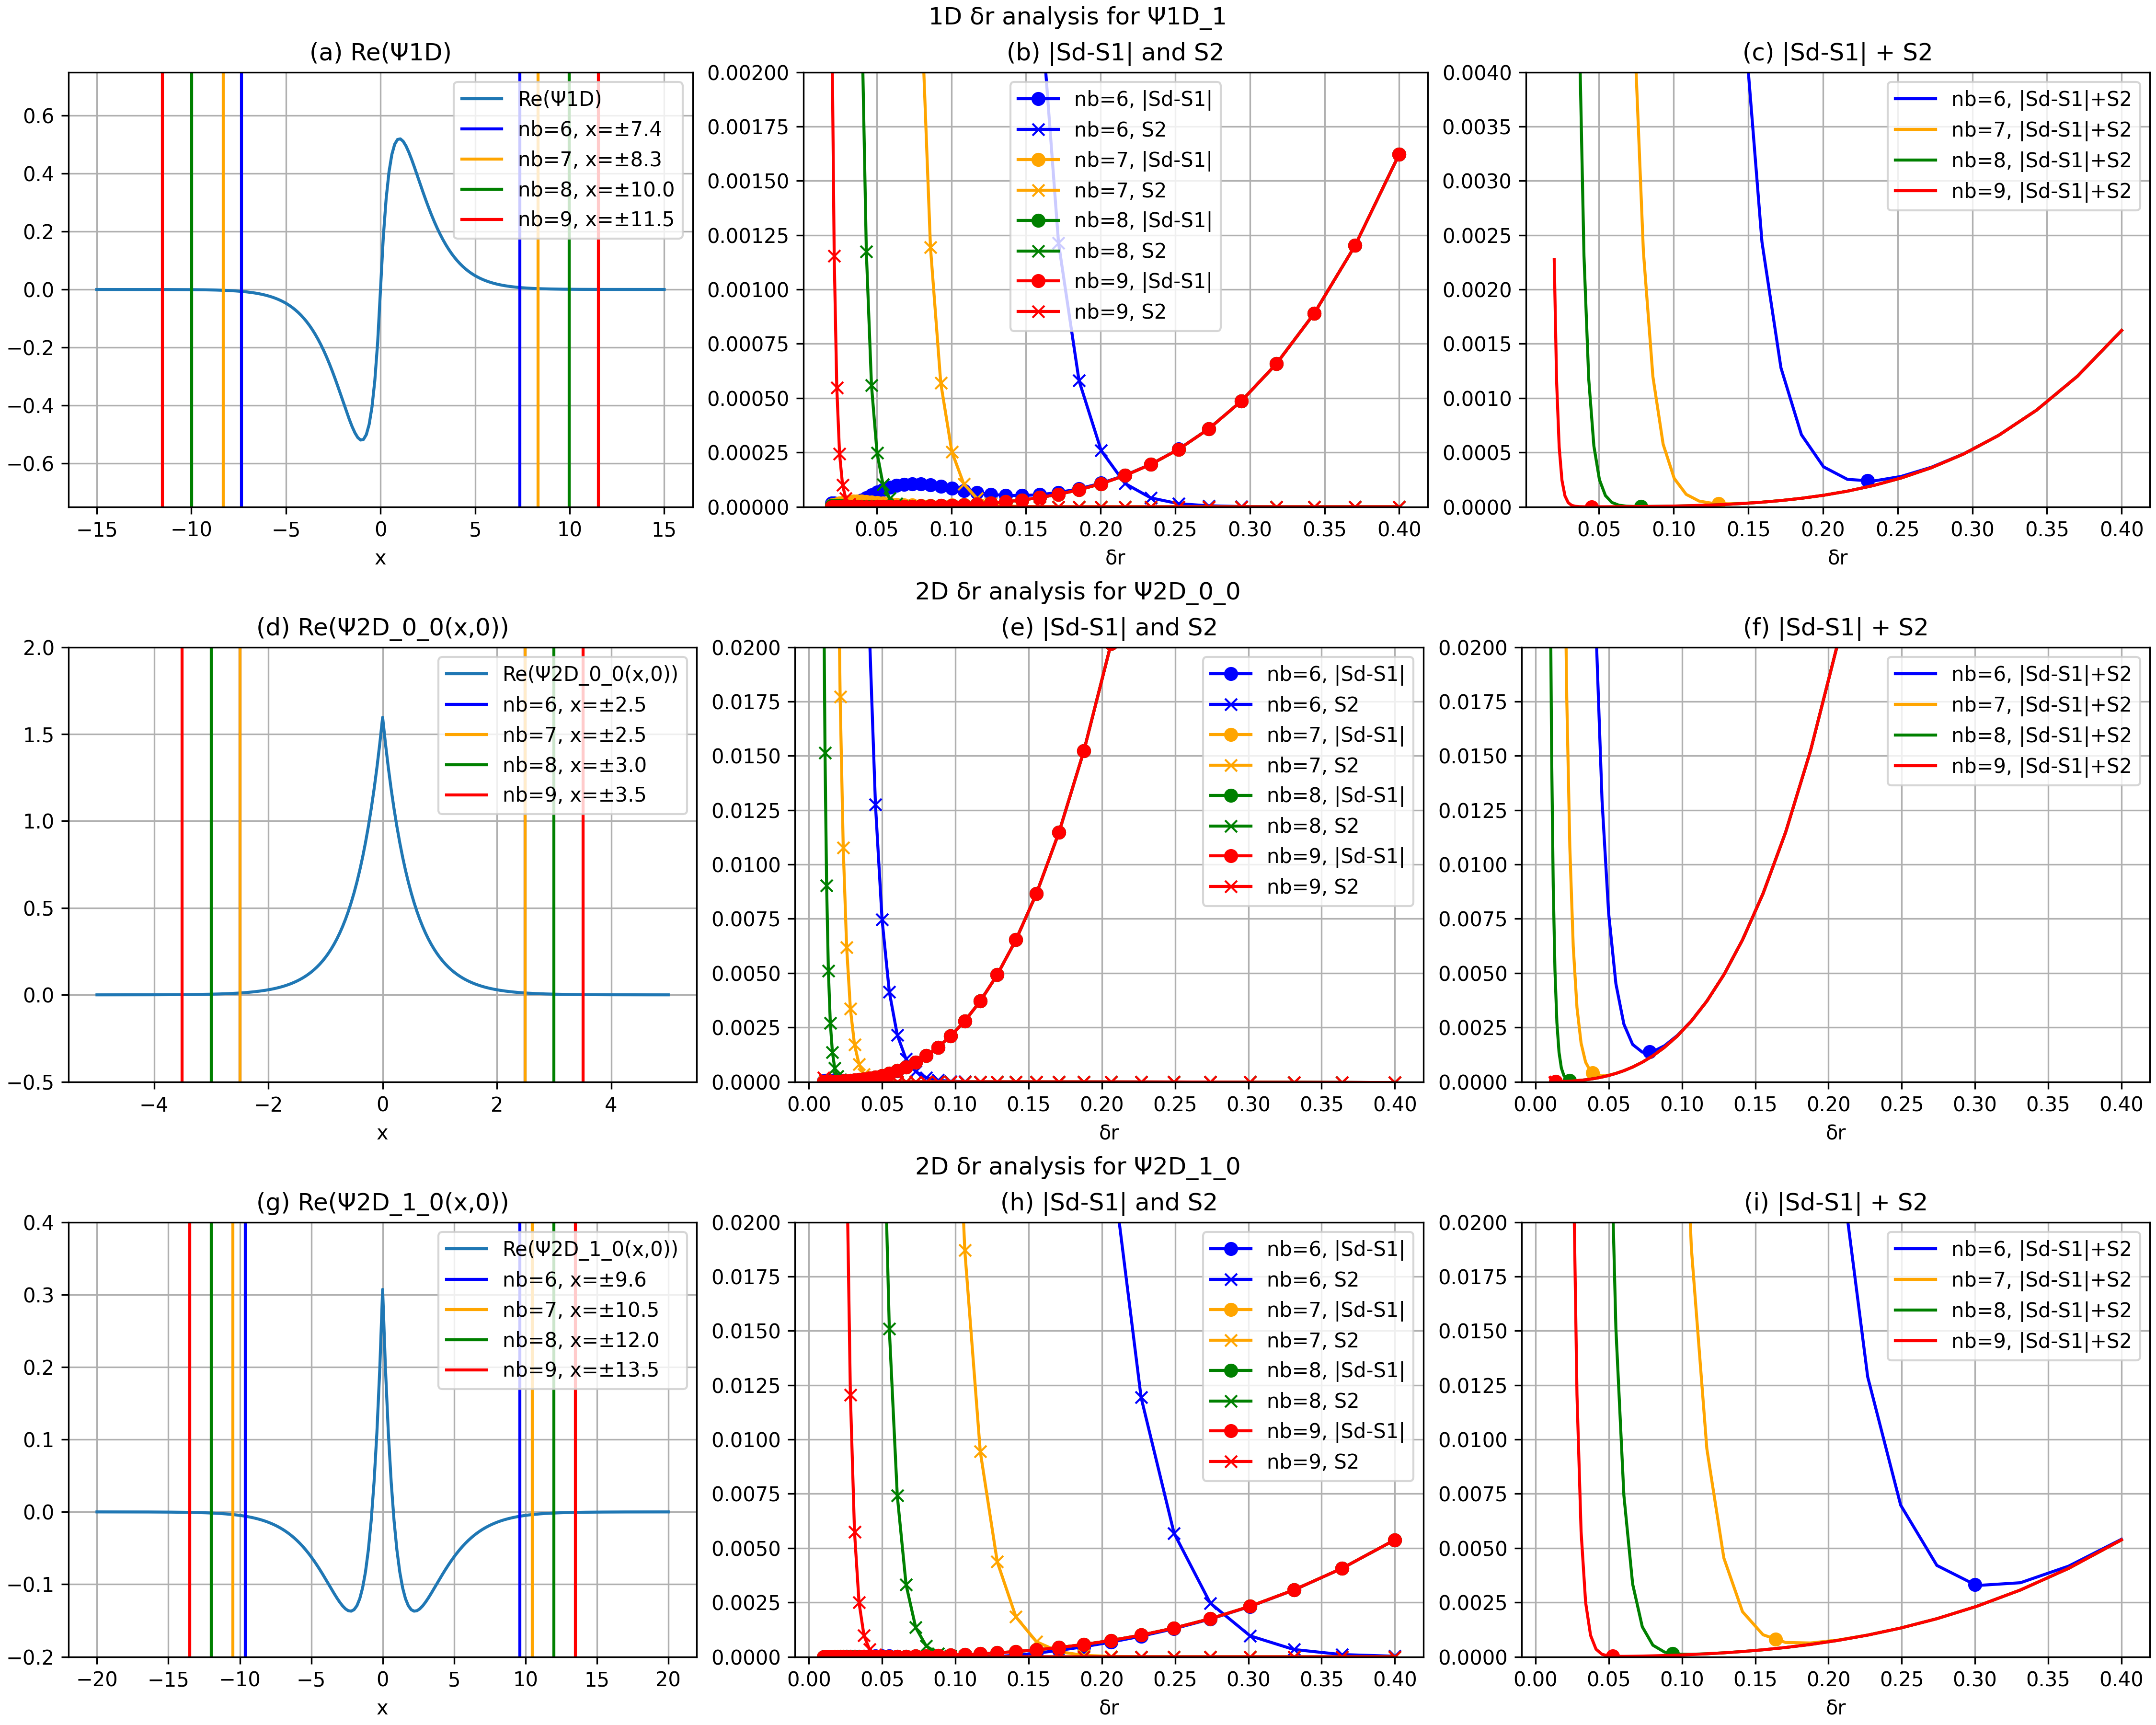
\includegraphics[width=\columnwidth]{paper2025_figs/dq_tradeoff/eval1d_2d.png}
    \caption{Relationship between $|\Sd-S_1|$ and $S_2$ at several $\nb$}
    \label{fig:dq-tradeoff}
    \begin{flushleft}\small 
        
        (a) shows the evaluation results for the 1D model $\PsiOneD_1$, and (b)
        and (c) show the results for the 2D model's $\PsiTwoD_{0,0}$ and
        $\PsiTwoD_{1,0}$, respectively. (A1) to (C1) show the real part values
        of the wave function at the intercept $y=0$ and the computational domain
        boundaries ($\pm L/2$) corresponding to the selected $\deltar$. (A2) to
        (C2) plot the discretization error and cutoff error individually, and
        (A3) to (C3) show their sum. The point where this sum of errors is
        minimized is the point of trade-off equilibrium, giving the optimal
        $\deltar$.

    \end{flushleft}
\end{figure}
\clearpage

\subsubsection{Conditions for Time Steps Based on the Sampling Theorem}
\label{subsubsec:deltat-selection-results}

Fixing the time evolution period to $t=1.0\ \mathrm{a.u.}$ (about $24.19\
\mathrm{as}$ in physical time), Figures \ref{fig:trotter-error-t1-part1} and
\ref{fig:trotter-error-t1-part2} show the relationship between the theoretical
upper bound of the error $\BN{\gamma}(\psi;t)$ and the actually observed
simulation error $\xiN{\gamma}$ when varying the number of Suzuki-Trotter
divisions $\nT$ ($\gamma=1,2$ indicates the Trotter order). Note that
considering the time evolution period of the wave function $\PsiTwoD_{1,0}$ is
$2\pi/E_2 \approx 28.27$, the evaluation results at $t=30$, which corresponds to
about one period, are deferred to the supplementary material
\ref{smsec:parameter-selection-for-minimum-error-analysis-details}.

Each graph indicates the lower limits of $\nT$ based on the sampling theorem,
$\nTpminTwoD$ and $\nTkminTwoD$, with vertical lines. The vertical axis is not
energy, but the norm of the difference in wave function amplitudes defined in
Equations \eqref{eq:observed-trotter-error-1st} and
\eqref{eq:observed-trotter-error-2nd}.

What is noteworthy is the difference in the effect of the Trotter order
depending on the quantum number of the target state. In the results for
$\PsiTwoD_{0,0}$ and $\PsiTwoD_{1,0}$ with an azimuthal quantum number of $m=0$
(Figure \ref{fig:trotter-error-t1-part1}(a) to (d)), no distinct difference in accuracy due
to the difference in the Trotter order $\gamma$ was observed. This is
consistent---despite the difference in dimensions---with the findings reported
by Burgarth et al. \cite{Burgarth2024.PhysRevResearch.6.043155}, who stated that
for 3D hydrogen atom models, increasing the Trotter order for eigenfunctions
with an azimuthal quantum number of 0 does not yield accuracy improvements.

On the other hand, in the results for $\PsiTwoD_{1,1}$ having an azimuthal
quantum number of $m=1$ (Figure \ref{fig:trotter-error-t1-part2}(a) and (b)), a clear difference in accuracy between
the 1st-order ($\xiN{1}$) and 2nd-order ($\xiN{2}$) Trotter decompositions can
be confirmed in the region where the number of divisions $\nT$ is small. This is
thought to be because the non-commutativity of kinetic energy and potential
energy has a stronger impact on states with angular momentum, causing the error
improvement effect of higher-order decomposition to appear more prominently.

As a general trend, under all conditions, the errors $\xiN{1}$ and $\xiN{2}$
decrease as the number of divisions $\nT$ increases, but the reduction saturates
near the lower limit for the kinetic energy term from the sampling theorem, $\nT
= \nTkminTwoD$. For $\PsiTwoD_{1,1}$, although a slight decrease in error is
seen even in the region of $\nT > \nTkminTwoD$, the practical impact is small.
This is because, upon reaching this region, the spatial discretization error
$\errdisc$ caused by the spatial resolution becomes more dominant than the time
error (Trotter error).

Therefore, under the conditions shown here, it can be said that setting the
number of divisions to far exceed the lower limit $\nTkminTwoD$ derived from the
sampling theorem only increases computational costs and does not contribute to
improving the overall error. Regarding the relationship with the spatial error,
this is evident, for example, when comparing Figure
\ref{fig:trotter-error-t1-part1}(a) ($\nb=6$) and Figure
\ref{fig:trotter-error-t1-part1}(b) ($\nb=9$). It can be confirmed that by
increasing the spatial resolution $\nb$, the floor of the residual error after
the Trotter error has saturated is significantly reduced to about 1/10.

\begin{figure}[ht]
    \centering
    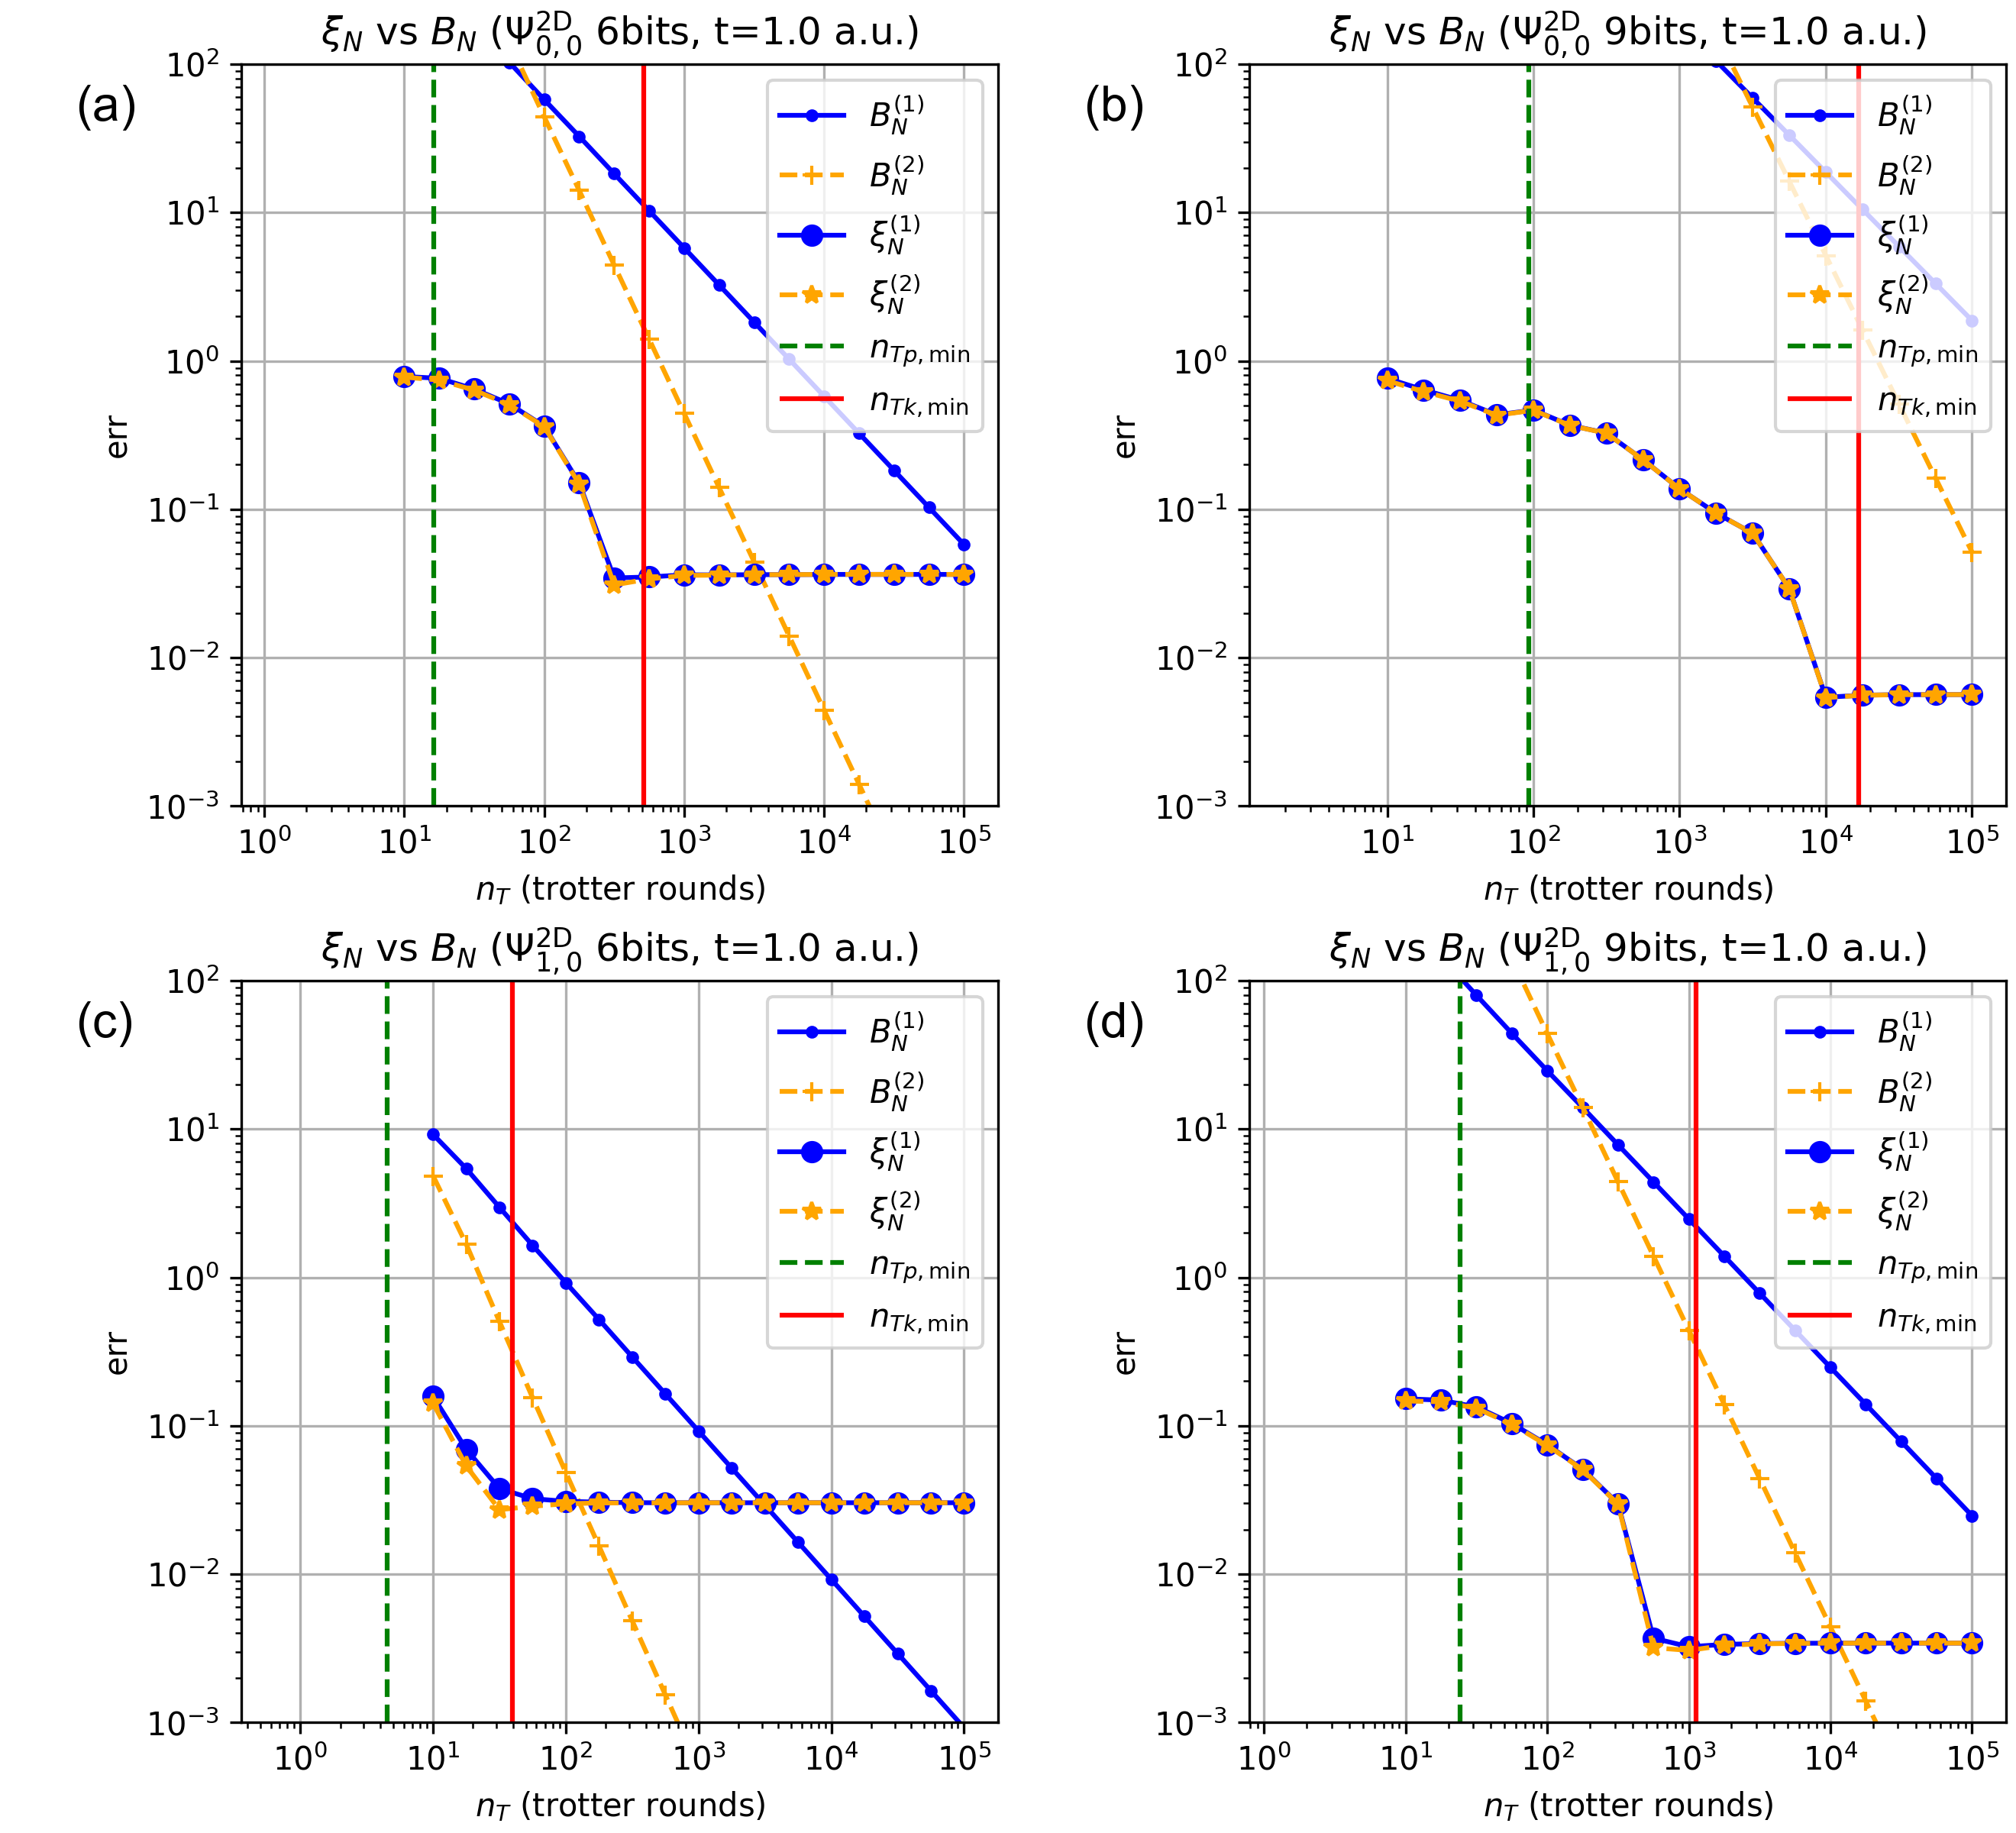
\includegraphics[width=\columnwidth]{paper2025_figs/sdt_error/trotter_err_00_10_t1.png}

    \caption{Upper bound $\BN{\gamma}$ and observed value $\xiN{\gamma}$ of the error with respect to the number of divisions $\nT$ at time evolution period $t=1.0$}
    \label{fig:trotter-error-t1-part1}
    \begin{flushleft}\small

        Relationship between the number of Trotter divisions and error in the 2D
        model. The time evolution period is fixed at $t=1.0$. $\xiN{1}$ and
        $\xiN{2}$ are the total observed errors (including spatial errors, etc.)
        from 1st- and 2nd-order Trotter decompositions, respectively. $\BN{1}$
        and $\BN{2}$ are the theoretically upper bound values of the Trotter
        error obtained analytically. The vertical lines $\nT=\nTpminTwoD$ and
        $\nT=\nTkminTwoD$ indicate the theoretical lower limits of the number of
        divisions for the potential term and kinetic energy term determined by
        the requirements of the sampling theorem.
    \end{flushleft}
\end{figure}

\begin{figure}[ht]
    \centering
    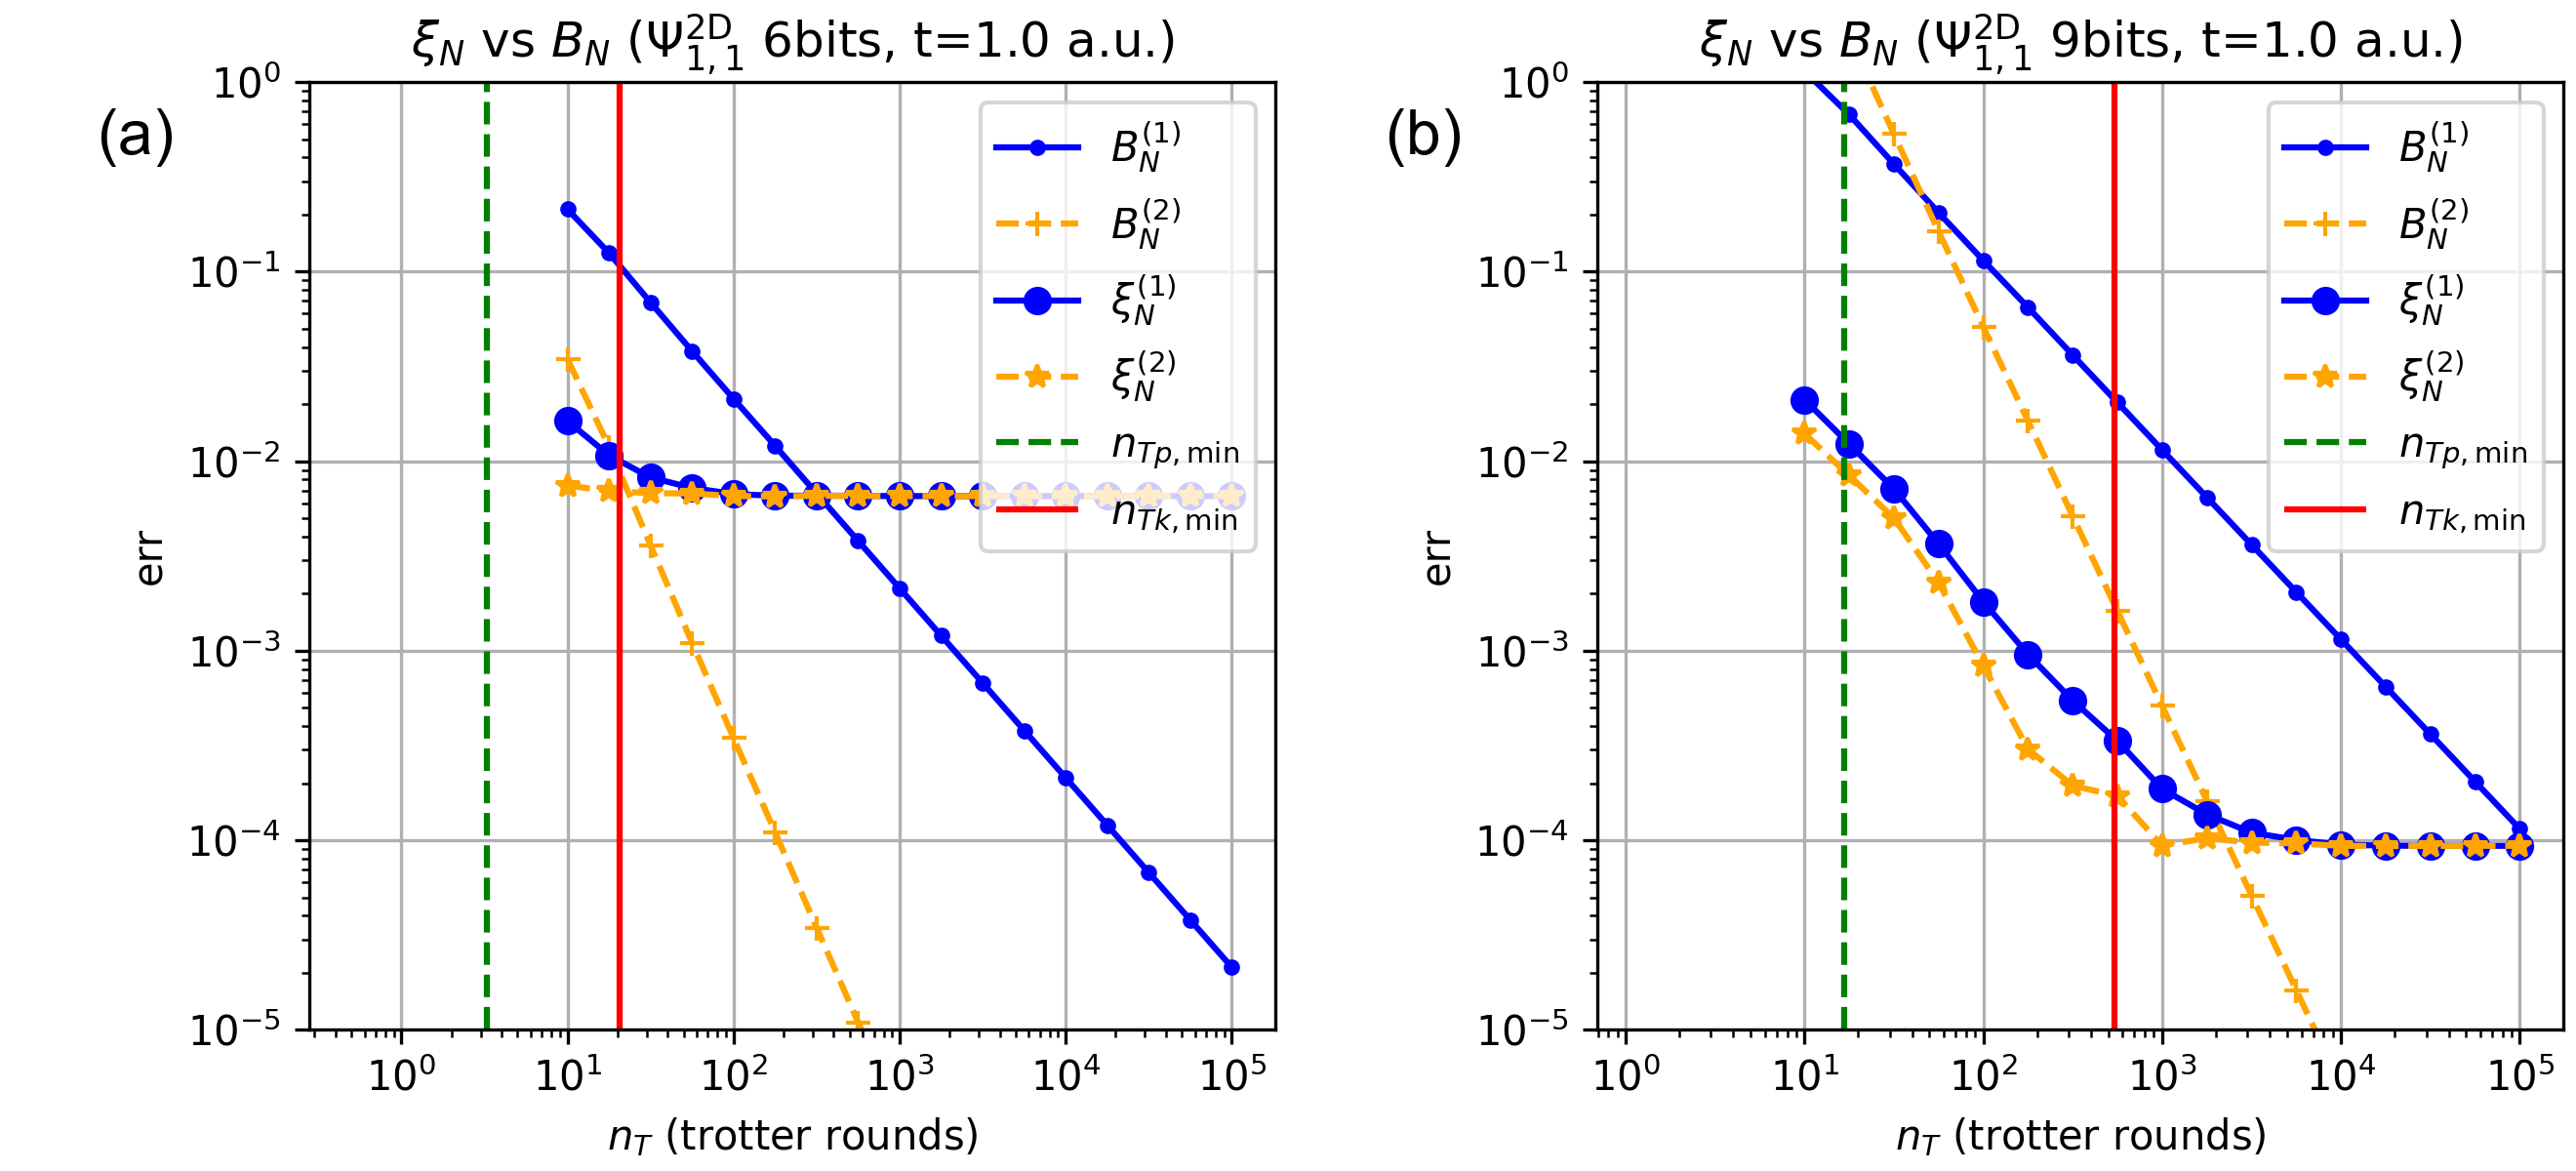
\includegraphics[width=\columnwidth]{paper2025_figs/sdt_error/trotter_err_11_t1.png}
    \caption{Upper bound $\BN{\gamma}$ and observed value $\xiN{\gamma}$ of the error with respect to the number of divisions $\nT$ at time evolution period $t=1.0$ (continued)}
    \label{fig:trotter-error-t1-part2}
    \begin{flushleft}\small

        Evaluation results for the wave function $\PsiTwoD_{1,1}$ with azimuthal
        quantum number $m=1$. In the region where $\nT$ is small, a significant
        difference in accuracy between the 1st- and 2nd-order Trotter
        decompositions is evident.
    \end{flushleft}
\end{figure}

\clearpage
\end{document}